% Preston Landers  <planders@utexas.edu>
% Master's Report document 
%
% Major: Computer and Electrical Engineering
% Focus: Software Engineering
% Cockrell School of Engineering
% The University of Texas at Austin
%
% Based on the UT LaTeX package provided at:
% http://www.utexas.edu/ogs/etd/LaTeX/



\documentclass[12pt]{report}	% The documentclass must be ``report''.

\usepackage{utdiss2}  		% Dissertation package style file.

%\usepackage[driver=pdftex,margin=1.2in,letterpaper]{geometry}
%\usepackage[driver=xetex,margin=1.2in,letterpaper]{geometry}

\usepackage{geometry}

\newenvironment{changemargin}[2]{%
\begin{list}{}{%
\setlength{\topsep}{0pt}%
\setlength{\leftmargin}{#1}%
\setlength{\rightmargin}{#2}%
\setlength{\listparindent}{\parindent}%
\setlength{\itemindent}{\parindent}%
\setlength{\parsep}{\parskip}%
}%
\item[]}{\end{list}}

%%%%%%%%%%%%%%%%%%%%%%%%%%%%%%%%%%%%%%%%%%%%%%%%%%%%%%%%%%%%%%%%%%%%%%
% Optional packages used for this sample dissertation. If you don't  %
% need a capability in your dissertation, feel free to comment out   %
% the package usage command.					     %
%%%%%%%%%%%%%%%%%%%%%%%%%%%%%%%%%%%%%%%%%%%%%%%%%%%%%%%%%%%%%%%%%%%%%%

\usepackage{amsmath,amsthm,amsfonts,amscd} 
				% Some packages to write mathematics.
\usepackage{eucal} 	 	% Euler fonts
\usepackage{verbatim}      	% Allows quoting source with commands.
\usepackage{makeidx}       	% Package to make an index.
\usepackage{graphicx}

\usepackage[hyphens]{url}		% Allows good typesetting of web URLs.

\usepackage{booktabs}  % table formatting
\newcommand{\ra}[1]{\renewcommand{\arraystretch}{#1}}
%\usepackage{float}
%\restylefloat{table}

\usepackage{caption}
\usepackage{subcaption}  % for sub-figures

\usepackage[backend=biber,url=false,citestyle=numeric,firstinits=false]{biblatex}
\usepackage{citesort}         	% 

\addbibresource{diss.bib}

% Prestons code listing definitions

% TODO: CUSTOM ELEMENTS (web components) are not recognized as HTML tags
% Add tags and attributes below as necessary.

% http://tex.stackexchange.com/questions/99500/listings-code-style-for-html5-css-html-javascript
% https://dl.dropboxusercontent.com/u/74217418/stackexchange/tex/html5_listings_sample.tex

\makeatletter
\usepackage{color}
\definecolor{lightgray}{rgb}{0.95, 0.95, 0.95}
\definecolor{darkgray}{rgb}{0.4, 0.4, 0.4}
\definecolor{purple}{rgb}{0.65, 0.12, 0.82}
\definecolor{editorGray}{rgb}{0.95, 0.95, 0.95}
\definecolor{editorOcher}{rgb}{1, 0.5, 0} % #FF7F00 -> rgb(239, 169, 0)
\definecolor{editorGreen}{rgb}{0, 0.5, 0} % #007C00 -> rgb(0, 124, 0)
\usepackage{upquote}
\usepackage{listings}
% CSS
\lstdefinelanguage{CSS}{
  keywords={color,background-image:,margin,padding,font,weight,display,position,top,left,right,bottom,list,style,border,size,white,space,min,width, transition:, transform:, transition-property, transition-duration, transition-timing-function},	
  sensitive=true,
  morecomment=[l]{//},
  morecomment=[s]{/*}{*/},
  morestring=[b]',
  morestring=[b]",
  alsoletter={:},
  alsodigit={-}
}

% JavaScript
\lstdefinelanguage{JavaScript}{
  morekeywords={typeof, new, true, false, catch, function, return, null, catch, switch, var, if, in, while, do, else, case, break},
  morecomment=[s]{/*}{*/},
  morecomment=[l]//,
  morestring=[b]",
  morestring=[b]'
}

\lstdefinelanguage{HTML5}{
  language=html,
  sensitive=true,	
  alsoletter={<>=-},	
  morecomment=[s]{<!-}{-->},
  tag=[s],
  otherkeywords={
  % General
  >, \{\{, \}\},
  % Standard tags
	<!DOCTYPE,
  </html, <html, <head, <title, </title, <style, </style, <link, </head, <meta, />,
	% body
	</body, <body,
	% Divs
	</div, <div, </div>, 
	% Paragraphs
	</p, <p, </p>,
	% scripts
	</script, <script,
  % More tags...
  <canvas, /canvas>, <svg, <rect, <animateTransform, </rect>, </svg>, <video, <source, <iframe, </iframe>, </video>, <image, </image>, <template, </template, <my-element, </my-element,
  <speakur-discussion, </speakur-discussion
  },
  ndkeywords={
  % General
  =,
  % HTML attributes
  charset=, src=, id=, width=, height=, style=, type=, rel=, href=,
  % SVG attributes
  fill=, attributeName=, begin=, dur=, from=, to=, poster=, controls=, x=, y=, repeatCount=, xlink:href=,
  % CSS properties
  margin:, padding:, background-image:, border:, top:, left:, position:, width:, height:,
	% CSS3 properties
  transform:, -moz-transform:, -webkit-transform:,
  animation:, -webkit-animation:,
  transition:,  transition-duration:, transition-property:, transition-timing-function:,
  }
}

\lstset{%
  % General design
  backgroundcolor=\color{editorGray},
  basicstyle={\small\ttfamily},   
  frame=l,
  % line-numbers
  xleftmargin={0.75cm},
  numbers=left,
  stepnumber=1,
  firstnumber=1,
  numberfirstline=true,	
  % Code design
  identifierstyle=\color{black},
  keywordstyle=\color{blue}\bfseries,
  ndkeywordstyle=\color{editorGreen}\bfseries,
  stringstyle=\color{editorOcher}\ttfamily,
  commentstyle=\color{darkgray}\ttfamily,
  % Code
  language=HTML5,
  alsolanguage=JavaScript,
  alsodigit={.:;},	
  tabsize=2,
  showtabs=false,
  showspaces=false,
  showstringspaces=false,
  extendedchars=true,
  breaklines=true,
  % German umlauts
  literate=%
  {Ö}{{\"O}}1
  {Ä}{{\"A}}1
  {Ü}{{\"U}}1
  {ß}{{\ss}}1
  {ü}{{\"u}}1
  {ä}{{\"a}}1
  {ö}{{\"o}}1
}

\makeatother



%\usepackage{xunicode}
%\usepackage[T1]{fontenc}
\usepackage{fontspec}
\usepackage{fixltx2e} % fix a problem with fnsymbol w/ fontspec, such as footnotes in vita

\usepackage[htt]{hyphenat}

% NOTE: technically the report formatting requirements say only
% a single font must be used. But I've seen many examples of 
% UT master's reports that use a monospace/teletype face for 
% technical terms. I believe that's considered a 'math font' so it's ok...

%\setmonofont[Scale=0.95]{Inconsolata}
%\setmonofont{Inconsolata}
%\usepackage{luximono}
%\usepackage[tt={oldstyle=true,variable=true}]{cfr-lm}
%\renewcommand{\ttdefault}{clmjv}

% My version of Inconsolata may not support bold/italic?
%\setmonofont[SmallCapsFont={Latin Modern Mono Caps}]{Latin Modern Mono Light}

\setmainfont[Ligatures=TeX]{Adobe Text Pro}
%\setmainfont[Ligatures=TeX]{Minion Pro}
\setmonofont[Scale=0.95]{Consolas}

%\usepackage{libertine}%% Only as example for the romans/sans fonts
%\usepackage{beraserif}
%\usepackage[scaled=0.9]{beramono}

\usepackage{hyperref}  % adds PDF bookmarks and such
\hypersetup{
 colorlinks=true,
 linkcolor=black,  % blue
 citecolor=black,  % green
 urlcolor=black,
% pdffitwindow=true,
 pdftitle={Speakur: Leveraging Web Components for Composable Applications},
 pdfauthor={Preston Landers <planders@utexas.edu>},
 pdfsubject={A case study in HTML5 Web Components, the Polymer framework, and Firebase.},
 pdfkeywords={Polymer} {Web Components} {HTML5} {Speakur} {Firebase},
 }
\hypersetup{breaklinks=true}
\usepackage{ragged2e}

\usepackage[capitalize]{cleveref}

% Force cleveref ``page'' references to be lowercase despite the capitalize option above
\crefformat{page}{page~#2#1#3}

% Set low penalties for breaks at numbers, uppercase letters and lowercase letters
\setcounter{biburlnumpenalty}{100}
\setcounter{biburlucpenalty}{100}
\setcounter{biburllcpenalty}{100}

% Fixes extra spacing around enumerate (bullet lists)
% http://stackoverflow.com/a/1073140/858289
\usepackage{enumitem}
\setlist{nolistsep}

%\pretolerance=10000

%\linespread{1.5} % Line spacing

%\usepackage{draftcopy}		% Uncomment this line to have the
				% word, "DRAFT," as a background
				% "watermark" on all of the pages of
				% of your draft versions. When ready
				% to generate your final copy, re-comment
				% it out with a percent sign to remove
				% the word draft before you re-run
				% Makediss for the last time.

\author{Preston Brent Landers}  	% Required

\address{\texttt{planders@utexas.edu} \\~\\ \url{https://github.com/Preston-Landers/} }  % Required

% Required
\title{Speakur: Leveraging Web Components \\ for Composable Applications}

%%%%%%%%%%%%%%%%%%%%%%%%%%%%%%%%%%%%%%%%%%%%%%%%%%%%%%%%%%%%%%%%%%%%%%
% NOTICE: The total number of supervisors and other members %%%%%%%%%%
%%%%%%%%%%%%%%% MUST be seven (7) or less! If you put in more, %%%%%%%
%%%%%%%%%%%%%%% they are put on the page after the Committee %%%%%%%%%
%%%%%%%%%%%%%%% Certification of Approved Version page. %%%%%%%%%%%%%%
%%%%%%%%%%%%%%%%%%%%%%%%%%%%%%%%%%%%%%%%%%%%%%%%%%%%%%%%%%%%%%%%%%%%%%

%%%%%%%%%%%%%%%%%%%%%%%%%%%%%%%%%%%%%%%%%%%%%%%%%%%%%%%%%%%%%%%%%%%%%%
%
% Enter names of the supervisor and co-supervisor(s), if any,
% of your dissertation committee. Put one name per line with
% the name in square brackets. The name on the last line, however,
% must be in curly braces.
%
% If you have only one supervisor, the entry below will read:
%
%	\supervisor
%		{Supervisor's Name}
%
% NOTE: Maximum three supervisors. Minimum one supervisor.
% NOTE: The Office of Graduate Studies will accept only two supervisors!
% 
%
%\supervisor
%	[Adnan Aziz]
%	{Johannes Kepler}
\supervisor
	{Adnan Aziz}

%%%%%%%%%%%%%%%%%%%%%%%%%%%%%%%%%%%%%%%%%%%%%%%%%%%%%%%%%%%%%%%%%%%%%%
%
% Enter names of the other (non-supervisor) members(s) of your
% dissertation committee. Put one name per line with the name
% in square brackets. The name on the last line, however, must
% be in curly braces.
%
% NOTE: Maximum six other members. Minimum zero other members.
% NOTE: The Office of Graduate Studies may restrict you to a total
%	of six committee members.
%
%
%\committeemembers
%	[Erwin Schr\"odinger]
%	[Albert Einstein]
%	[Charles Townes]
%	{Arthur Schawlow}
\committeemembers
	{Christine Julien}


%%%%%%%%%%%%%%%%%%%%%%%%%%%%%%%%%%%%%%%%%%%%%%%%%%%%%%%%%%%%%%%%%%%%%%

\previousdegrees{B.A.}
     % The abbreviated form of your previous degree(s).
     % E.g., \previousdegrees{B.S., MBA}.
     %
     % The default value is `B.S., M.S.'

\graduationmonth{May}
     % Graduation month, either May, August, or December, in the form
     % as `\graduationmonth{May}'. Do not abbreviate.
     %
     % The default value (either May, August, or December) is guessed
     % according to the time of running LaTeX.

\graduationyear{2015}
     % Graduation year, in the form as `\graduationyear{2001}'.
     % Use a 4 digit (not a 2 digit) number.
     %
     % The default value is guessed according to the time of 
     % running LaTeX.

%\typist{...}       
     % The name(s) of typist(s), put `the author' if you do it yourself.
     % E.g., `\typist{Maryann Hersey and the author}'.
     %
     % The default value is `the author'.


%%%%%%%%%%%%%%%%%%%%%%%%%%%%%%%%%%%%%%%%%%%%%%%%%%%%%%%%%%%%%%%%%%%%%%
% Commands for master's theses and reports.			     %
%%%%%%%%%%%%%%%%%%%%%%%%%%%%%%%%%%%%%%%%%%%%%%%%%%%%%%%%%%%%%%%%%%%%%%
%
% If the degree you're seeking is NOT Doctor of Philosophy, uncomment
% (remove the % in front of) the following two command lines (the ones
% that have the \ as their second character).
%
\degree{Master of Science in Engineering}
\degreeabbr{M.S.E.}

% Uncomment the line below that corresponds to the type of master's
% document you are writing.
%
\masterreport
%\masterthesis


%%%%%%%%%%%%%%%%%%%%%%%%%%%%%%%%%%%%%%%%%%%%%%%%%%%%%%%%%%%%%%%%%%%%%%
% Some optional commands to change the document's defaults.	     %
%%%%%%%%%%%%%%%%%%%%%%%%%%%%%%%%%%%%%%%%%%%%%%%%%%%%%%%%%%%%%%%%%%%%%%
%
%\singlespacing
%\oneandonehalfspacing

%\singlespacequote
\oneandonehalfspacequote

\topmargin 0.125in	% Adjust this value if the PostScript file output
			% of your dissertation has incorrect top and 
			% bottom margins. Print a copy of at least one
			% full page of your dissertation (not the first
			% page of a chapter) and measure the top and
			% bottom margins with a ruler. You must have
			% a top margin of 1.5" and a bottom margin of
			% at least 1.25". The page numbers must be at
			% least 1.00" from the bottom of the page.
			% If the margins are not correct, adjust this
			% value accordingly and re-compile and print again.
			%
			% The default value is 0.125"

		% If you want to adjust other margins, they are in the
		% utdiss2-nn.sty file near the top. If you are using
		% the shell script Makediss on a Unix/Linux system, make
		% your changes in the utdiss2-nn.sty file instead of
		% utdiss2.sty because Makediss will overwrite any changes
		% made to utdiss2.sty.

%%%%%%%%%%%%%%%%%%%%%%%%%%%%%%%%%%%%%%%%%%%%%%%%%%%%%%%%%%%%%%%%%%%%%%
% Some optional commands to be tested.				     %
%%%%%%%%%%%%%%%%%%%%%%%%%%%%%%%%%%%%%%%%%%%%%%%%%%%%%%%%%%%%%%%%%%%%%%

% If there are 10 or more sections, 10 or more subsections for a section,
% etc., you need to make an adjustment to the Table of Contents with the
% command \longtocentry.
%
%\longtocentry 



%%%%%%%%%%%%%%%%%%%%%%%%%%%%%%%%%%%%%%%%%%%%%%%%%%%%%%%%%%%%%%%%%%%%%%
%	Some math support.					     %
%%%%%%%%%%%%%%%%%%%%%%%%%%%%%%%%%%%%%%%%%%%%%%%%%%%%%%%%%%%%%%%%%%%%%%
%
%	Theorem environments (these need the amsthm package)
%
%% \theoremstyle{plain} %% This is the default

\newtheorem{thm}{Theorem}[section]
\newtheorem{cor}[thm]{Corollary}
\newtheorem{lem}[thm]{Lemma}
\newtheorem{prop}[thm]{Proposition}
\newtheorem{ax}{Axiom}

\theoremstyle{definition}
\newtheorem{defn}{Definition}[section]

\theoremstyle{remark}
\newtheorem{rem}{Remark}[section]
\newtheorem*{notation}{Notation}

%\numberwithin{equation}{section}


%%% Preston custom macros
\newcommand{\tcode}[1]{\texttt{#1}}

%%%%%%%%%%%%%%%%%%%%%%%%%%%%%%%%%%%%%%%%%%%%%%%%%%%%%%%%%%%%%%%%%%%%%%
%	Macros.							     %
%%%%%%%%%%%%%%%%%%%%%%%%%%%%%%%%%%%%%%%%%%%%%%%%%%%%%%%%%%%%%%%%%%%%%%
%
%	Here some macros that are needed in this document:


\newcommand{\latexe}{{\LaTeX\kern.125em2%
                      \lower.5ex\hbox{$\varepsilon$}}}

\newcommand{\amslatex}{\AmS-\LaTeX{}}

\chardef\bslash=`\\	% \bslash makes a backslash (in tt fonts)
			%	p. 424, TeXbook

\newcommand{\cn}[1]{\texttt{\bslash #1}}

\makeatletter		% Starts section where @ is considered a letter
			% and thus may be used in commands.
\def\square{\RIfM@\bgroup\else$\bgroup\aftergroup$\fi
  \vcenter{\hrule\hbox{\vrule\@height.6em\kern.6em\vrule}%
                                              \hrule}\egroup}
\makeatother		% Ends sections where @ is considered a letter.
			% Now @ cannot be used in commands.

\makeindex    % Make the index


%%%%%%%%%%%%%%%%%%%%%%%%%%%%%%%%%%%%%%%%%%%%%%%%%%%%%%%%%%%%%%%%%%%%%%
%		The document starts here.			     %
%%%%%%%%%%%%%%%%%%%%%%%%%%%%%%%%%%%%%%%%%%%%%%%%%%%%%%%%%%%%%%%%%%%%%%

\begin{document}

\copyrightpage          % Produces the copyright page.


%
% NOTE: In a doctoral dissertation, the Committee Certification page
%		(with signatures) is BEFORE the Title page.
%	In a masters thesis or report, the Signature page
%		(with signatures) is AFTER the Title page.
%
%	If you are writing a masters thesis or report, you MUST REVERSE
%	the order of the \commcertpage and \titlepage commands below.
%
\commcertpage           % Produces the Committee Certification
			%   of Approved Version page (doctoral)
			%   or Signature page (masters).
			%		20 Mar 2002	cwm

\titlepage              % Produces the title page.



%%%%%%%%%%%%%%%%%%%%%%%%%%%%%%%%%%%%%%%%%%%%%%%%%%%%%%%%%%%%%%%%%%%%%%
% Dedication and/or epigraph are optional, but must occur here.      %
%%%%%%%%%%%%%%%%%%%%%%%%%%%%%%%%%%%%%%%%%%%%%%%%%%%%%%%%%%%%%%%%%%%%%%
%
\begin{dedication}
\index{Dedication@\emph{Dedication}}%
This report is dedicated to my wife for her patience,\linebreak
and to my parents for their support and guidance
\end{dedication}


\begin{acknowledgments}		% Optional
\index{Acknowledgments@\emph{Acknowledgments}}%
I would like to thank Bill Balcezak for strongly encouraging and facilitating the completion of my undergraduate and graduate education. 
I would also like to thank Curt Finch, John Maddalozzo and everyone else at Journyx for their patience, understanding and encouragement.

I would also like to thank my supervisor, Dr. Adnan Aziz, 
for his enthusiasm, invaluable feedback, wisdom, and for teaching one of best classes I've ever taken.
In addition I would like to thank Dr. Christine Julien, Mr. Bill Bard, Dr. Kathleen Barber, and all of the other excellent instructors in the CLEE program.
Without this amazing program and everyone mentioned above, I would not be who I am today.
\end{acknowledgments}


% The abstract is required. Note the use of ``utabstract'' instead of
% ``abstract''! This was necessary to fix a page numbering problem.
% The abstract heading is generated automatically.
% Do NOT use \begin{abstract} ... \end{abstract}.
%
\utabstract
\index{Abstract}%
\indent

This report is a case study of applying abstraction, encapsulation, and composition techniques to web application architecture with the use of Web Components, 
a proposed extension to the HTML5 Document Object Model. 
I created Speakur, a real-time social discussion plugin for the mobile and desktop web, 
to show how Web Components can help realize software engineering principles and design patterns, including the composition of applications from components sourced from diverse authors and frameworks.

Web authors can add a Speakur discussion to their page by inserting a simple HTML element at the desired spot to give the page a real-time discussion or feedback system.
Speakur uses the Polymer framework's implementation of the draft Web Components standard to achieve the encapsulation of its internal implementation details from the containing page behind a simplified, well defined interface.
Web Components are a proposed W3C standard for writing custom HTML tags that take advantage of new browser technologies like Shadow DOM, package importing, CSS Flexboxes and data-bound templates.

This report reviews Web Components and related technologies and provides a case study for structuring a real-world WC applet that is embedded in a larger app or system.
The major research question is whether Web Components offer a viable path towards the encapsulation and composition principles that have largely eluded web engineers thus far. 
In other words, \textit{are components really the future of the web}? 
Subsidiary topics include assessing the maturity and performance of current Web Components technologies,
and methods of synchronization between user interface components and local and remote data models.
My analysis shows that Web Components successfully address many of the key structural and organizational problems faced by web software engineers.

\tableofcontents   % Table of Contents will be automatically
                   % generated and placed here.

\listoftables      % List of Tables and List of Figures will be placed
\listoffigures     % here, if applicable.
\lstlistoflistings


%%%%%%%%%%%%%%%%%%%%%%%%%%%%%%%%%%%%%%%%%%%%%%%%%%%%%%%%%%%%%%%%%%%%%%
% Actual text starts here.					     %
%%%%%%%%%%%%%%%%%%%%%%%%%%%%%%%%%%%%%%%%%%%%%%%%%%%%%%%%%%%%%%%%%%%%%%
%
% Including external files for each chapter makes this document simpler,
% makes each chapter simpler, and allows for generating test documents
% with as few as zero chapters (by commenting out the include statements).
% This allows quicker processing by the Makediss command file in case you
% are not working on a specific, long and slow to compile chapter. You
% can even change the chapter order by merely interchanging the order
% of the include statements (something I found helpful in my own
% dissertation).
%
\chapter{Introduction}
\index{Introduction@\emph{Introduction}}%

%\section{blah}
%\index{blah@\emph{blah}}%
%
%\texttt{asdf}
%
%\begin{quote}
%\index{guarantee}%
%This template package is provided and licensed ``as is'' without warranty
%of any kind, either expressed or implied, including, but not limited to,
%the implied warranties of merchantability and fitness for a particular
%purpose. Yadda, yadda, yadda, \ldots
%\end{quote}

This report presents a case study of applying W3C Web Components 
\index{Web Components}
to achieve encapsulation and modularity within the context of collaborative web authoring. 
The author has created Speakur, a real-time discussion social plugin for the web, 
as an experiment to determine the maturity and viability of using Web Components to create modern, highly composable web applications.

Like most web applications, Speakur is written in HTML markup and Java\-script code. 
HTML is a declarative markup language used to create documents --- web pages --- which are viewed with the help of a program called the browser. 
The Hyper\-text Markup Language (HTML) 
\index{HTML}
standard has proven wildly successful since its introduction in 1993 by British computer scientist 
Tim Berners-Lee, 
\index{Tim Berners-Lee}
with billions and billions of pages served, 
and millions of public and private web sites forming a major part of our information landscape. [CITE?]
More than any other invention, other than perhaps email, the World Wide Web (WWW) has shaped how we see and use the global network.

% 
\begin{figure}[htb]
\centering
 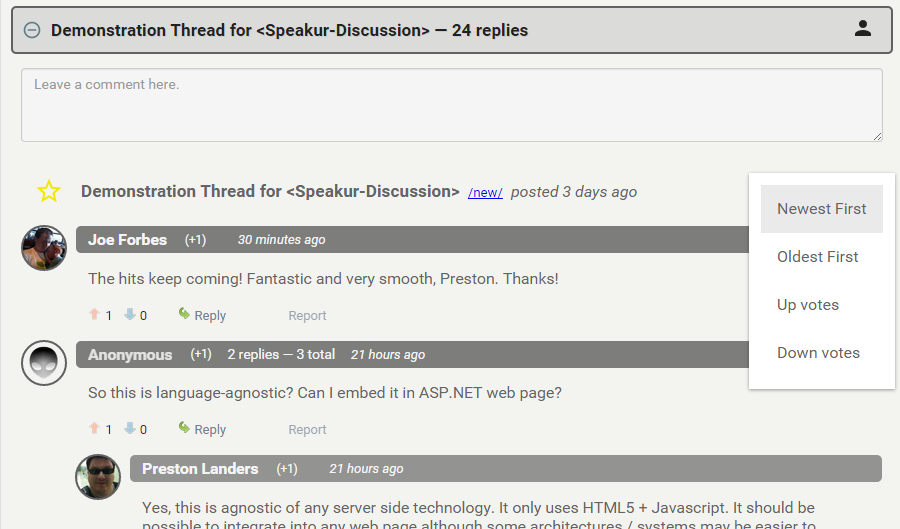
\includegraphics[width=6in]{images/screenshot_20150312_1630_v2.png}
\caption{A Speakur thread inside a demonstration page.}
\label{f:demo1}
\end{figure}
\index{commands!environments!figure}%

Those designing and programming applications for the Web as a computing platform have long dreamed of the ability to mix and match independent, reusable chunks of functionality --- components --- in their documents without mutual coupling and interference. 
The original and current Document Object Model (DOM)
\index{DOM}
browser abstraction provided by HTML does not allow for significant decoupling; 
everything lives together on one big page. Hacks like the 
\tcode{<iframe>} 
\index{iframe}
tag have allowed one to work around some of these restrictions, 
usually in a limited and inelegant way.

At the time of HTML's introduction the concept of quickly and easily composing a static web page, 
much less a full-fledged dynamic application, 
out of Lego-like reusable building blocks seemed like a distant dream at best. 
The introduction of the 
Javascript\footnote{Javascript, also rendered as JavaScript or JS, 
has no significant relation to Sun's (now Oracle's) popular Java programming language;
the name is an unfortunate coincidence at best.

To complicate the naming situation even further, Javascript is officially standardized under the name ECMAScript (ES).}
\index{Javascript}
(JS) programming language to web browsers in 1995 allowed for a completely new dimension of dynamic behavior that was not possible before.
Eventually web apps powered by Javascript like Gmail and Google Docs rivaled traditional desktop applications in functionality and usability while being instantly accessible from nearly anywhere.
Still, web apps had to be stitched together `by hand' in ways that carefully ensured that the different parts didn't step on each other's toes, else disaster frequently ensued. 
Each component or area of the system could not help but be coupled to the others at some level as a result of the programming model imposed by the DOM and HTML.

Over the years the dynamic behaviors afforded by Javascript grew in importance along with the web, and helped contribute to its success. 
The flexible, loosely typed nature of Javascript aided the prototyping process and initial development,
but the difficulties of maintaining a semblance of coherence in a large sprawling application soon became apparent.
Over time a bewildering array of frameworks and libraries sprang up around the HTML/JS ecosystem to help manage this complexity and to provide scaffolding and structure for client side web apps.
For many years individual JS frameworks seemed to come and go as ephemerally as teenage pop idols. 
The industry kept searching for the Next Big Thing that would make writing high quality web apps less of bug-ridden, messy chore. 

In recent years (roughly 2011 to 2014) Google's Angular [CITE] 
\index{Angular}
has emerged as a dominant client framework, 
due in part to its high perceived quality [CITE] and the fact that it represents an common point for a fragmented industry to rally around.
Facebook's React 
\index{React}
JS library with its Virtual DOM is an up-and-comer focused on high performance that is more complementary in nature to Angular than a true challenger.

Yet despite the emergence of the updated HTML5 standard in 2011 and the recent successes of web frameworks like Angular and React in capturing developer attention, 
there still did not exist a clear picture of how web apps could achieve the encapsulated component model that had become prevalent in other areas of software engineering.
That is, until engineers from Google\footnote{
As of March 2015, Google's Chrome browser is the most popular desktop browser. [CITE]}
\index{Google}
and Mozilla\footnote{
The Mozilla Foundation is the sponsor of the popular Firefox web browser. It grew out of Netscape, whose Navigator browser helped bring the web to a mass audience.}
\index{Mozilla} 
and other organizations got together [\textbf{WHEN?}] to draft a new standard called \textbf{Web Components} that will extend and enhance HTML5 in ways that could have a significant long-term impact.

\section{Web Components Overview}
Fundamentally, the Web Components standard consists of four new core DOM technologies --- extensions to the current HTML5 standard.
If these standards are accepted by major browser vendors and the World Wide Web Consortium (W3C)
\index{W3C}
which maintains HTML, 
they will eventually become native browser features and available directly to any web page without needing to use any additional JS frameworks or libraries. 
The core Web Component technologies are:
\begin{itemize}
\item
\textbf{Custom Elements}: extending HTML with author-created tags
\item
\textbf{Shadow DOM}: encapsulation for the internals of custom elements
\item
\textbf{Templates}: scaffolding for instantiating blocks of HTML from inert templates
\item
\textbf{Imports}: packaging for HTML components
\end{itemize}

This report also explores several related web standards initiatives that are frequently associated with Web Components 
but are not formally grouped under them, including mutation observers,
\index{mutation observers}
model driven views, 
\index{model driven views}
and the CSS Flexible Boxes
\index{Flex box} 
and CSS Grid
\index{CSS Grid}
systems. 
Because these technologies are not yet formally accepted as W3C standards and are not yet widely implemented in typical mobile and desktop browsers, 
Speakur has been implemented using Google's experimental Polymer framework [CITE].
Polymer provides a Javascript `polyfill'
\index{polyfill}
library to implement many of the new Web Component features in browsers which would otherwise not support them. 
Eventually this platform polyfill should become unnecessary, in theory, as WC becomes widely adopted in browsers.
Some browsers like Google Chrome already have at least some native Web Component support and on these browsers the polyfill is effectively a `no-op'.

The potential componentization of the web is one of the most exciting developments in web engineering in years and follows the overall growth in software-as-a-service (SaaS) 
\index{SaaS}
and the service oriented architecture
\index{Service Oriented Architecture}
model. 
The conversion of dynamic web logic---not mere snippets of plain HTML---into bundles of reusable, extendable, composable components enables web developers to move to a higher level of abstraction than was previously possible.

The move towards a component-based Web will enable interesting new composite services, mashups, and may help broaden the potential pool of web developers. 
What previously required a highly integrated, high-overhead development model or lots of tedious glue code can become as simple as importing a custom element and dropping it onto a page.


\section{Structure of This Report}
\index{Structure of This Report@\emph{Structure of This Report}}%

The goal of this report is to demonstrate the application of software engineering design patterns embodied in the  W3C proposed Web Components standard such as encapsulation, modular composition, and automatic synchronization of application state. 
This report discusses many of the goals and principles of the Web Components initiative and how a number of different technologies taken together help raise the overall level of abstraction for content authors, web engineers, and application developers --- which I will refer to collectively as (web) authors for short.

The Background section provides an introduction to some of the architectural problems inherent in modern web authoring and how Web Components (WC) address them. 
It also provides some background on software engineering design patterns that are embodied in Web Components such as encapsulation, composition, and inheritance, as well as technologies such as WebSockets and NoSQL databases.
It describes some of the motivations behind the development of Speakur and some of the specific software engineering questions it addresses, such as the ability to provide a hassle-free way to host an embedded discussion forum inside an arbitrary web resource in a way that is fully encapsulated.

The Approach section details the specific structures and techniques used when constructing a Web Component, and describes the technology and software architecture choices that went into Speakur. 
It describes how Speakur uses Web Components to implement encapsulated modules whose internals are protected from unintentional outside influence.

The Implementation section describes the application of Web Component principles to the specific task of providing a flexible and suitably generic discussion forum / commenting plugin for both desktop and mobile browsers. 
It describes the overall architecture, code flow, and synchronization process.
An important topic in this section is security: how can we implement a largely client-based system while maintaining some kind of data integrity?

This is followed by an Analysis section which discusses some of the outcomes as compared to the original goals and also looks at the impact of the selection of Web Components, Polymer, Firebase and some of the other architectural choices. 
A few quantitative results are included, I hope \textbf{(TODO)}.

Finally, the Conclusion section is just all kinds of awesome and wraps up the report \textbf{(TODO)}. 

\section{Source Code and Demonstration Resources}
\index{Source Code and Demonstration Resources@\emph{Source Code and Demonstration Resources}}%

The source code for Speakur consists of HTML and Javascript files located in a Git version control repository. 
These files constitute an ``HTML Import'' package that provides a
\textbf{\tcode{<speakur-discussion>}}
custom HTML element for the use of web authors in their own pages.

% XXX TODO: bold around \tcode has no effect?
% http://tex.stackexchange.com/questions/215482/how-do-i-get-texttt-with-bold-face-in-latex

The Speakur source code and component documentation can be found here on GitHub.com:

\tcode{\url{https://github.com/Preston-Landers/speakur-discussion}}

Demonstrations of several web pages which show off embedded Speakur discussions are available at the following location:

\tcode{\url{https://preston-landers.github.io/speakur-discussion/components/speakur-discussion/demo.html}}


\chapter{Background}
\index{Background%
@\emph{Background}}%
\label{ch:background}

When the Web was first created by Tim Berners-Lee\index{Berners-Lee, Tim} in 1989, web pages were largely envisioned as static \textit{documents} with a single author or a small group of coordinating authors. 
The idea of composing a complex web application out of basic components like snapping together Lego blocks seemed like a distant dream at best.
Until recently, web authors were limited to using the predefined HTML layout elements or `tags' that were listed in the W3C standard and understood by browser programs, such as \tcode{<title>} and \tcode{<video>}. 
Creating your own \textit{sui generis} HTML elements with unique behaviors seemed beyond the capabilities of the web browsers of the day like Mosaic\index{Mosaic}
and Netscape Navigator\index{Netscape Navigator}.

As of early 2015, modern web apps are typically written with a JavaScript\index{JavaScript} framework that provides a cohesive set of structures, design patterns and practices designed to facilitate composing web applications 
--- large or small --- 
from a number of sub-com\-ponents~\cite{dickey2014}.
Angular\index{Angular}, Meteor\index{Meteor}, and Backbone\index{Backbone} are three such frameworks.
The difference between a `framework'\index{framework} and a library is somewhat arbitrary, but typically frameworks are more comprehensive than narrowly focused utility libraries.
Yet all frameworks must exist within the confines of the programming model provided by the browser and the Document Object Model (DOM)\index{DOM}. 
In this model, the entire web page or app belongs to a single `document', constituent parts are not encapsulated\index{encapsulation} or isolated from each other, and authors are limited to working with the predefined HTML tags.
These issues make it difficult to create and share generic, reusable \textit{web components} 
--- in the abstract sense --- 
among different users who may not use the same frameworks or follow the same set of assumptions and conventions.

\section{Current challenges in web authoring}
In object oriented programming, encapsulation\index{encapsulation} is typically defined as a 
``language mechanism for restricting access to some of the object's components''
~\cite[p. 522]{mitchell2003}.
The point of encapsulation is providing an \textit{abstraction} that consumers of the functionality can rely on without knowing the internals. 
The goals of encapsulation and abstraction include:
\begin{quote}
Identifying the interface of a data structure~\dots~providing \textit{information hiding} by separating implementation decisions from parts of the program that use the data 
structure~\dots~and allowing the data structure to be used in many different ways by many different components~\cite[p. 243]{mitchell2003}.
\end{quote}

Although techniques of abstraction\index{abstraction} and encapsulation\index{encapsulation} have been widespread in object oriented programming for decades,
the fundamental web client programming model has not allowed for significant encapsulation of things like the DOM structure and CSS style rules~\cite{ihrig2012}.
To illustrate how these problems affect the ability of authors to share and reuse code, let's look at an example from the popular Twitter\index{Twitter} Bootstrap\index{Bootstrap} library~\cite{bootstrapcontributors2015}.
Twitter Bootstrap is a collection of Cascading Style Sheet (CSS)\index{CSS} rules and JavaScript\index{JavaScript} widgets or components designed to allow web authors to quickly `bootstrap' an attractive, consistent look-and-feel onto a web page.
Bootstrap provides pre-styled user interface\index{user interface (UI)} (UI) widgets such as menus, buttons, panels, dropdown selectors, alerts, dialogs, and so on, to be used as building blocks to construct web sites or application user interfaces.
Because Bootstrap must work within the confines of the DOM\index{DOM} and the HTML5\index{HTML!HTML5} standard, this necessarily exposes a great deal of Bootstrap's internals to its users.
For example, to add a Bootstrap site navigation bar to your page, you must essentially copy and paste a large block of HTML\index{HTML} and then customize it to your needs as shown in Figure~\ref{f:twbs1}.

\begin{figure}[htb]
\centering
 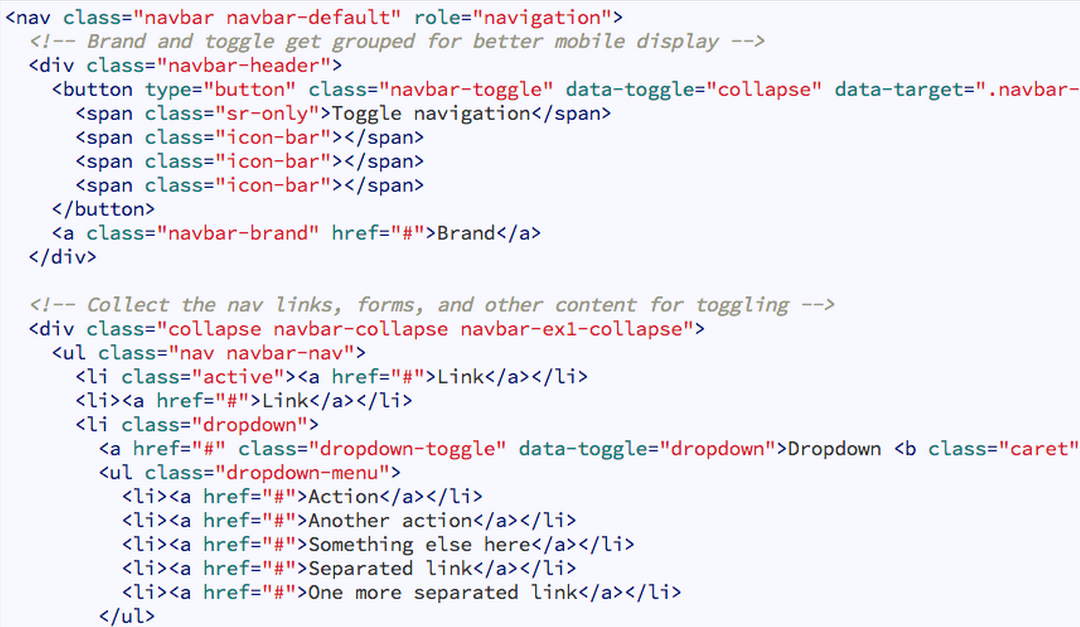
\includegraphics[width=\textwidth]{images/bootstrap_navbar_html.png}
\caption{Partial example of Twitter\index{Twitter} Bootstrap\index{Bootstrap} navigation bar HTML.}
\label{f:twbs1}
\end{figure}


This forces Bootstrap's\index{Bootstrap} users to tightly couple the layout of their page with the internal structure required by Bootstrap's navigation bar widget. 
This coupling hinders a significant refactoring\index{refactoring} of the navigation widget's internal structure (HTML\index{HTML} layout) because that would require the large community of developers to update their applications accordingly.
In addition, because CSS\index{CSS} rules normally apply across the entire page, the authors of Bootstrap must carefully select the scope and nomenclature of all rules to ensure no unintended side-effects~\cite{walton2014}. 
Even then, conflicts are inevitable when the entire page is treated as a single sandbox and you combine components from many different vendors. 

What if instead one could create and share a reusable chunk of functionality --- a web component -- that hid all of these tedious structural details and encapsulated its private, internal state? 
What if web authors could create their \textit{own} HTML elements?  
Using Bootstrap's navigation bar could be as easy as replacing the code in Figure~\ref{f:twbs1} with a custom element like the one in the following example:

% 
%\begin{figure}[htb]
%\centering
% 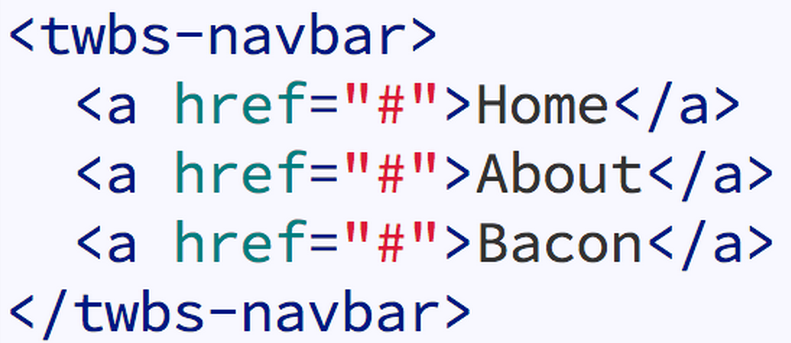
\includegraphics[width=3.5in]{images/bootstrap_navbar_wc.png}
%\caption{Hypothetical Bootstrap nav bar custom element.}
%\label{f:twbs2}
%\end{figure}

\begin{lstlisting}[language=HTML5,caption={Hypothetical Bootstrap nav bar custom element.},label=l:twbs2]
 <twbs-navbar>
   <a href="#">Home</a>
   <a href="#">About</a>
   <a href="#">Sign In</a>
 </twbs-navbar>
\end{lstlisting}

\subsection{Abstraction, encapsulation and composition}

The Web Components working group, consisting of software engineers\index{software engineering} from several major browser vendors, 
looked at this situation and found that, in practice, browsers already had a suitable model for encapsulating components that hide complexity behind well-defined interfaces.
That model was that one used internally by browsers to implement the newer 
HTML5\index{HTML!HTML5} tags 
like the \textbf{\tcode{<video>}} element.\index{<video>} 
The \tcode{<video>} element presents a simple interface (API) to HTML authors that hides the complexities of playing high definition video.
Internally, however, browsers implement \tcode{<video>} with a `shadow' or hidden document inside the object that contains the internal state~\cite{kitamura2014}. 
For example, an author can write:
\begin{lstlisting}[language=HTML5,numbers=none]
	<video loop src=...> </video>
\end{lstlisting}
to cause the video to loop repeatedly.

\begin{figure}[htb]
%\centering
\centerline{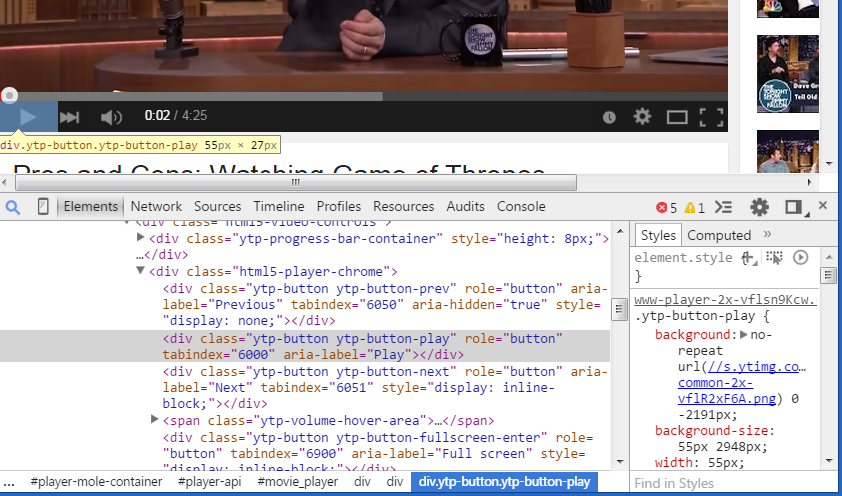
\includegraphics[width=6in]{images/html5_video_control.png}} 
\caption{Opera's\index{Opera} shadow DOM for \tcode{<video>}\index{<video>} highlighting the Play button}
\label{f:html5video}
\end{figure}

This shadow\index{Shadow DOM} Document Object Model (DOM)\index{DOM} inside the 
\tcode{<video>}\index{<video>} tag creates the user interface (UI) needed to control video playback such as the volume controls, the timeline bar, and the pause and play buttons.
These inner playback controls are themselves built out of HTML, CSS\index{CSS} and JS but these details are not exposed to web authors who simply place a \tcode{<video>} element on their page. 
Figure~\ref{f:html5video} illustrates how this works. It shows the shadow (internal) DOM of a \tcode{<video>} element on a page with the Play button \tcode{<div>} highlighted.
A small \tcode{\#player-api} tag is visible in the DOM path at the bottom of Figure~\ref{f:html5video}.
This is an example of the container inside \tcode{<video>}\index{<video>} using the abstraction of a \tcode{\#player-api} to encapsulate the details of actually controlling playback within the context of the overall \tcode{<video>} interface.

This example illustrates three component design principles that are widely followed in other areas of software engineering\index{software engineering}~\cite{fowler2012}:
\begin{itemize}
\item Create layers of \textbf{abstraction}\index{abstraction} to represent `public' details that are relevant to the surrounding code or environment.
\item Use \textbf{encapsulation}\index{encapsulation} and well defined interfaces to protect private state, hide implementation complexity, and leave implementors free to refactor internals.
\item Prefer \textbf{composition}\index{composition} or \textit{has-a} relationships over inheritance or \textit{is-a} relationships when building modules to reduce coupling and simplify interface refactoring\index{refactoring}.
\end{itemize}

Composition helps reduce coupling or structural between modules by forcing them to interact using only public interfaces.
In the case of the interface for \tcode{<video>}, it's composed of simple block elements and scoped CSS\index{CSS} roles and the Volume and Play controls aren't particularly special objects, just \tcode{<divs>} with CSS rules and click handlers.

The solution, therefore, to these coupling problems in web authoring is to expose these internal brower APIs for creating elements in a safe and portable fashion. 
This will allow web authors to create their own rich custom elements using standard portable APIs, encapsulate their internals, and enable easier sharing, composition and integration.
The question remains, which specific browser internals must be exposed and standardized in order to support Web Components?

\section{Web Components}

Web Components consists of two main technologies and two supporting features. 
Custom HTML Elements\index{Custom Elements} and Shadow DOM\index{Shadow DOM} are the two key players while HTML Imports\index{HTML!Imports} and Templates\index{HTML!Templates} support these features. 
One of the central goals of the Web Components\index{Web Components} initiative is to maintain interoperability across different browsers and frameworks, 
so that modules which adhere to the Web Components standard can provide a consistent experience no matter what framework the developer chooses or which browser the user selects.
For example, an important benefit of Custom Elements is that they \textit{are} standard HTML elements; they live in the DOM\index{DOM} and can be accessed by the usual DOM methods and the majority of standard HTML/JS development tools~\cite{penades2015}.
They also behave somewhat like objects in traditional object oriented programming (OOP) in that 
they have \textit{methods} and hidden internal \textit{state} (data).

\subsection{Custom HTML elements}
Never before have web authors been able to define their own custom HTML elements\index{Custom Elements} that were not found in the official list.
Actually, many authors and web frameworks have been doing exactly that for years, primarily for internal purposes where the custom elements are pre\-processed and compiled down to standard HTML.
The custom elements would not get sent to the end user's browser because it would not know what to do with them.
In addition, the DOM\index{DOM} has long supported creating custom-named elements, but it was not possible to do much interesting with them because they were treated like an ordinary 
\tcode{<span>}\index{<span>} element~\cite{w3ccontributors2015-b}.
However, the possibility now exists to create custom elements in a standard way that will work consistently across browsers with the W3C Custom Element\index{Custom Elements}
specification~\cite{w3ccontributors2015-b}. 

The primary restriction is that all custom elements must have a \texttt{-} character (dash) in their name, such as \tcode{<my-element>}. 
This is to avoid a name collision with future built-in HTML elements. 
To create a new Custom Element, you must first register the element:

\begin{lstlisting}[language=JavaScript,numbers=none]
 var MyElement = document.registerElement('my-element');
\end{lstlisting}

Then you can place your new element on the page, either declaratively in HTML:

\begin{lstlisting}[language=HTML5,numbers=none]
 <my-element> hello, world! </my-element>
\end{lstlisting}

or imperatively with JavaScript\index{JavaScript}:

\begin{lstlisting}[language=JavaScript,caption={Registering a custom element\index{Custom Elements} in JavaScript\index{JavaScript}.},label=l:register]
 var MyElement = document.registerElement('my-element');

 // create a new instance of the element
 var thisOne = new MyElement();      
 document.body.appendChild(thisOne); // add to the <body>
\end{lstlisting}

In a small example like this, the result does not look all that different in the browser from a \tcode{<span>}.
To do something more interesting with your custom element you will need to the other features of Web Components: Shadow DOM, templates and imports.

\subsection{Shadow DOM}
\label{bg:shadowdom}
Shadow DOM\index{Shadow DOM} encapsulates the internal structure of an element~\cite{w3ccontributors2015}. 
As we have seen, browsers already use Shadow DOM to encapsulate the private state of standard elements like \tcode{<video>}\index{<video>} but now this capability is extended to custom-defined elements.

You can think of shadow DOM like an HTML fragment inside an element that describes its external appearance without exposing these structural details\footnote{
HTML5 Shadow~DOM\index{Shadow DOM} should not be confused with the React\index{React} framework's \textbf{Virtual}~DOM, which is conceptually closer to HTML5 Templates in nature than Shadow DOM.}. 
Typically a custom element definition has a template (more on these later) which produces the shadow DOM necessary to render the element.
The actual contents of the shadow DOM are just ordinary elements.
Any element, whether custom or not, can have zero, one, or more shadow DOM trees attached.

Custom elements can wrap regular text, normal HTML elements, other custom elements, or nothing at all,
and then project that content through its shadow DOM, 
therefore into its visual representation.
In the example in Listing~\ref{l:twbs2} above, 
a \textbf{\tcode{<twbs-navbar>}} element consumes a set of three 
\textbf{\tcode{<a>}} (anchor or link) elements but internally transforms that to something like the example in Figure~\ref{f:twbs1}, 
projecting the set of links into the nav menu structure with appropriate wrappers.

The \tcode{<content>}\index{<content>} tag is used inside a custom element's template to indicate the spot where the consumed (wrapped) content should be \textit{projected}. 
This wrapped content is known as 
\textit{light DOM}\index{Light DOM}, 
because it's given by the user and projected through into the shadow.
Together the shadow DOM and light DOM form the \textit{logical DOM}\index{Logical DOM} of a custom element.
It is also possible for elements to have multiple shadow DOM sub-trees. 
This is used particularly for emulating object-oriented-like inheritance relationships between custom elements.

In languages like C\#\index{C\# language} and Java\index{Java}, the encapsulation\index{encapsulation} of classes and the protection of private object fields are a relatively strong guarantee by the language.
JavaScript\index{JavaScript} variables can be protected by \textit{closures}\index{closure}
but shadow DOM and CSS\index{CSS} are not completely and utterly isolated from the containing page.
It is possible to ``reach inside'' and break encapsulation to at least some degree, 
but the point is that this must be an intentional act by the developer and not an unexpected side-effect~\cite{bidelman2014}.

\subsection{HTML Imports}
One significant problem faced by web developers is the lack of any built-in packaging system for modules in HTML.
Prior to Web Components there was no way to import a snippet of HTML or JavaScript\index{JavaScript} from an external location and insert it exactly one time into the current document, 
similar to an \tcode{\#include}\index{\tcode{\#include}} directive in the C language\index{C language} or the packaging and import systems that are popular in scripting languages\index{scripting languages}
like Python\index{Python language}, Go\index{Go language} and Ruby\index{Ruby language}. 
JavaScript can always be loaded with a \tcode{<script>} tag\index{<script>} like usual, but this does not ensure that resources are loaded and executed exactly once, a process known as \textit{de-duping}\index{de-duping}.
A component that uses a certain JS resource might be needed in two different spots on the page, 
but that resource would be requested twice and executed twice, degrading application performance.

In order to fix these problems the HTML Imports\index{HTML!Imports} standard allows for bringing in snippets of HTML, CSS\index{CSS} or JavaScript into the current document in a way that ensures automatic de-duping of repeated requests~\cite{w3ccontributors2015-a}.
The one major caveat is that de-duping only happens if the resources are named in exactly the same fashion in each case~\cite{bidelman2013}.
Dealing with HTML Imports in a consistent fashion is discussed in section~\ref{sec:dependencies}.

\subsection{Templates}
The last major piece of the Web Component puzzle is the native HTML5\index{HTML!HTML5} \tcode{<template>}\index{<template>} tag. 
Unlike the rest of Web Components, \tcode{<template>} has already become a standard part of the HTML5 specification, 
although one that is perhaps not widely used yet outside of WC~\cite{w3ccontributors2015-c}.
\textit{Template} is a frequently overloaded word with different meanings in different programming environments.
While HTML5 templates have some similarities to the concept of templates popularized by frameworks\index{framework} like Angular\index{Angular} and Django\index{Django framework}, there are some important differences.

HTML5\index{HTML!HTML5} templates are inert hunks of HTML embedded in the page that can be instantiated into `real' elements by JavaScript\index{JavaScript}.
Their basic function is to give a source input for the shadow DOM\index{Shadow DOM} when you create a new (custom) element instance and place it on the page.
However, templates are most useful in combination with `live' data, not static, unchanging text.
Binding data into templates with special operators\footnote{
Sometimes called mustaches, handlebars or curly braces. },
also known as a Model-Driven View\index{Model-Driven View},
is \textbf{not} a part of the standard HTML5\index{HTML!HTML5} template spec.
The following example of a data bound template is something that does \textit{not} work with plain Web Components alone:

\begin{lstlisting}[language=HTML5,caption={An example of a data-bound template.},label=l:dbtemplate]
	<template> 
		The temperature is {{ temp }} in {{ city }} right now.
	</template>
\end{lstlisting}

Google\index{Google} engineers have advanced a proposal for standardizing 
Model-Driven Views\index{Model-Driven View}
but it is not yet part of the standard \tcode{<template>}\index{<template>} element~\cite{googledevelopers2014}.
Instead this functionality can be handled by a JavaScript\index{JavaScript} framework such as React or Polymer.
Data-bound templates are discussed in more detail in the following chapters.

The primary benefit of HTML Templates\index{HTML!Templates} from a performance perspective is that external resources referenced from the template (images, stylesheets, etc.) will not be fetched until the template is actually instantiated.
Templates are often used to declare the internal structure (shadow DOM\index{Shadow DOM}) of custom elements. 
Therefore the resources needed to use the custom element\index{Custom Elements} aren't downloaded until they are actually needed, which is necessary when composing a large application out of numerous distinct components, 
not all of which are needed immediately.

\section{Related W3C initiatives}
There are a number of related W3C\index{W3C} initiatives for web standards. 
Sometimes these are loosely grouped under the label Web Components,
and they do support componentization in web application design, 
but they are a separate part of the HTML5\index{HTML!HTML5} standard.
These include mutation observers\index{mutation observers}, 
DOM\index{DOM} selectors\index{Selectors}, 
and so-called `responsive' attributes designed to adjust the layout automatically according to screen size.
All of these techniques have been used extensively in Speakur\index{Speakur}.

\subsection{Mutation Observers}
\label{sec:bgmutation}
For example, \textit{mutation observers}\index{mutation observers}
allow a component to register a `callback'\index{callback} function to observe and react to any changes in the state of an area of interest in the DOM\index{DOM}, 
whether that change was generated by a user action or another 
component~\cite{w3ccontributors2014}.
This helps decouple components by allowing them to react asynchronously\index{asynchronous} to changes in each other's public state without directly interconnecting the components with bound variables.
The observers ``deliver mutations in batches asynchronously\index{asynchronous} at the end of a micro-task rather than immediately after they occur''~\cite{addyosmani2014}.
This improves the user experience (UX)\index{user experience (UX)} by ensuring that the callback\index{callback} is only called as-needed rather than once for each small change.

\subsection{Selectors}
\label{sec:bgselectors}
Another standardization initiative is in the area of DOM\index{DOM} / CSS\index{CSS} \textit{selectors}\index{Selectors},
as popularized by the highly successful jQuery\index{jQuery} library
written by John Resig,\index{Resig, John} 
which as of 2012 was used in half of all major websites~\cite{matthiasgelbmann2012}.
The Selector\index{Selectors} API was officially standardized in 2013 and browser support is good in current versions~\cite{w3ccontributors2013}.

The JS selector API allow you to quickly find DOM elements based on a rule-based description string (the selector) to perform further operations on their state such as reading or modifying data, observing future changes, attaching animations, and so on. 
The following example shows how to populate a JS variable with the element that has the \tcode{id} attribute equal to \tcode{some-id}:

\begin{lstlisting}[language=JavaScript,caption={JavaScript query selector example.}]
	// find an element whose id is equal to 'some-id'
	var someElem = document.querySelector("#some-id");
	if (someElem) console.log("Found it!");
	else console.log("Wasn't there.");
\end{lstlisting}


%Pointer events:

% \url{http://www.w3.org/TR/pointerevents/}

% Web animations:

% \url{http://www.w3.org/TR/web-animations/}

% Selectors  (similar to jQuery selectors)

% rl{http://www.w3.org/TR/selectors-api/}


%\textit{Placeholder Notes}:
%A significant problem with 'web components' story - scoping!  
%There is just one global scope on the page.
%This leads to the practice of 'prefixing as poor man's scope'.  
%E.g. instead of facebook providing a <like-button> element, they provide <facebook-like-button>.
%apparently this may be an area of future development  (citation?)

\subsection{Responsive layout for mobile}

The rise of smartphones and other mobile\index{mobile} devices has accelerated the need for web developers to make their applications responsive to the type of client used to access it.
Creating a web site or application that adjusts to the smaller screen of a mobile phone is often known as \textit{responsive design}\index{responsive design}.
Before the addition of responsive design features to the HTML\index{HTML} spec, 
it was always possible to make manual layout adjustments in JavaScript\index{JavaScript} but this was sometimes brittle and error-prone.

Besides JavaScript\index{JavaScript}, at least three CSS techniques can be used to make a responsive design: 
the \tcode{@media}\index{@media} rule, 
the Grid\index{Grid} layout, 
and Flexible (Flex)\index{Flex} boxes.
The CSS \tcode{@media}\index{@media} rule allows one to restrict the scope of CSS rules such that they only apply to certain media types including different screen sizes.

The CSS Grid layout is primarily intended to control the overall page layout on different device sizes~\cite{w3ccontributors2015-d}.
For example, a 'sidebar' might normally run alongside the main content down the side of the page in a desktop layout, but in a mobile layout the sidebar might come down at the end after the main content.
This includes different layouts for portrait vs. landscape device orientation.
The CSS Flexible Boxes model (Flex)\index{Flex} is intended for adjusting the flow of smaller page components~\cite{mozillacontributors2015}.
Flex boxes are useful for general user interface\index{user interface (UI)} (UI) structure, not just device-responsive design, and are widely used in Polymer\index{Polymer} and in Speakur\index{Speakur}~\cite{polymercontributors2015-d}.

\section{Polymer framework}

The exciting possibilities offered by Web Components seemed to call for a new framework engineered from the ground-up to take advantage of it.
In light of that, a team within Google\index{Google} developed the 
Polymer\index{Polymer} framework both to embody the Web Components\index{Web Components} 
architecture\index{architecture}~\cite{polymercontributors2015} and 
to provide a suite of components and user interface widgets useful for building applications.
Because Web Components are a bleeding-edge feature not yet natively implemented in most browsers,
the Polymer developers opted to create a \textit{polyfill}\index{polyfill}, 
library to fill in these missing features to the degree possible.
This polyfill is used in several other Web Components related projects such as 
X-Tags\index{X-Tags}~\cite{x-tagscontributors2015} and Bosonic~\cite{bosoniccontributors2014}\index{Bosonic}.
Unfortunately polyfills cannot provide a 100\% complete Web Components implementation; 
only native browser support can.

Because Polymer\index{Polymer} and to a lesser extent Web Components are still experimental and under development, 
they are both subject to frequent changes.
The version of Speakur\index{Speakur} described in this report is based on Polymer release 0.5.
As of the time of this writing, Polymer 0.8 is planned and will contain significant breaking changes to application structure~\cite{michaelbleigh2015}.
Small portions of this report pertaining to specific Polymer\index{Polymer} practices or interfaces are likely to be out of date by the time you read this.

\section{Speakur}
My desire to learn more about modern web development led me to investigate web frameworks like Angular\index{Angular} and Meteor\index{Meteor}.
I built elementary demos with these two frameworks in particular.
Although they certainly let you `get stuff done', and are used every day to power high-traffic applications, 
I was unhappy with the non-standard and idiosyncratic nature of these frameworks. 
They relied on `proprietary' (even if open source) extensions that were not native to HTML\index{HTML} and not easily transportable across different frameworks and architectures\index{architecture}.
This dissatisfaction led me to learn about the Web Components\index{Web Components} initiative.

\subsection{Origin}
Learning about Web Components quickly led me to the Polymer\index{Polymer} project.
I wanted to create something that demonstrated common use cases for Web Components and also showed off some of the design possibilities provided by Polymer and 
Material Design~\cite{imura2015}\index{Material Design}.
I was also intrigued by the possibilities of a server-free design afforded by Firebase\index{Firebase}.
Some kind of `live' social plugin seemed like a natural fit for the capabilities of Polymer and Firebase, so this led to a discussion plugin for blogs and other articles.
My hope was that it would required little or nothing in the way of dedicated server resources in order for other web authors to actually use it. 

\subsection{Motivations}
\label{motivations}
I wanted my discussion component to have some of the following attributes:

\begin{enumerate}
\item A simple API and usage pattern that abstracted\index{abstraction} away most of the implementation details.\label{motive:abstraction}

\item Require minimal server resources. Ideally nothing would need to be ``installed'' and it could be loaded in a cross-origin fashion from online developer tools like \url{https://jsbin.com}.
\label{motive:cors}

\item Event notification for changes similar to the 
publish-subscribe\index{publish-subscribe} (pubsub) design pattern.\label{motive:pubsub} 
For example, automatically updating when new replies are posted or existing posts are edited.

\item Support Markdown\index{Markdown} formatted comments including syntax highlighting for code snippets.\label{motive:markdown}

\item Support 
internationalization\index{internationalization}
(i18n) and 
localization\index{localization} (l10n) features for a global audience.\label{motive:i18n}

\item If any framework was used at all, it should be based on Web Components\index{Web Components}.\label{motive:webcomponents} This ruled out the vast majority of frameworks, 
leaving only Polymer\index{Polymer} and the less-comprehensive X-Tags\index{X-Tags}~\cite{x-tagscontributors2015} and Bosonic~\cite{bosoniccontributors2014}\index{Bosonic} projects and a few other less ambitious contenders.

\end{enumerate}

The next chapter discusses some of the high level architectural concerns that should be addressed when designing this type of social web plugin, such as creating a scalable database schema, designing a device-responsive user interface, and providing authentication and authorization rules.

\chapter{Approach}
\index{Approach%
@\emph{Approach}}%

\section{Functionality}

\section{Architecture Overview}
Roy Fielding, the influential author of the REST web architecture, wrote that

\begin{quote}
a software architecture is an abstraction of the run-time elements of a software system during some phase of its operation. A system may be composed of many levels of abstraction and many phases of operation, each with its own software architecture.

At the heart of software architecture is the principle of abstraction: hiding some of the details of a system through encapsulation in order to better identify and sustain its properties. A complex system will contain many levels of abstraction, each with its own architecture.~\cite{fielding2000}
\end{quote}


\section{Responsive Design}

\section{Polymer and Web Components}

\section{Data store and synchronization}
\subsection{NoSQL and Firebase}

'Serverless'

\subsection{Web Sockets}

\subsection{Security}

\section{Data Flow and Event Handling}

\subsection{Mutation Observers}

\section{Dependencies and Deployment}

Bower

Vulcanize

CORS



\chapter{Implementing a Web Component}
\index{Implementing a Web Component%
@\emph{Implementing a Web Component}}%
\label{ch:implementation}

\section{Overview}
\label{ch4:overview}
Speakur\index{Speakur} is an HTML5\index{HTML!HTML5} web application that uses the Polymer\index{Polymer} framework's implementation of Web Components\index{Web Components}.
It is primarily a client side application with no dedicated server component other than Firebase\index{Firebase}.
It is delivered as a single Custom Element\index{Custom Elements}, \tcode{<speakur-discussion>}\index{<speakur-discussion>}.
You import the tag with \tcode{<link rel=import href=...>} to make it available to place on the page. 
This element has a data-bound\index{data-bound template} \tcode{<template>}\index{<template>} that provides the element's visual representation (shadow DOM).
Actually, a custom element's representation, or logical DOM\index{Logical DOM}, may consist of both encapsulated shadow DOM\index{Shadow DOM} as well as light DOM\index{Light DOM} that is supplied by the \textit{user} of the custom element and \textit{projected} into the shadow DOM as discussed in~\cref{bg:shadowdom}.
In Speakur's case, the discussion forum is self-contained in terms of content; light DOM is not needed or used in the top-level element.
Speakur's\index{Speakur} options or parameters are controlled with attributes\index{HTML!attributes} like this:

\begin{lstlisting}[language=HTML5,caption=
{Using HTML attributes to set Speakur options.},label=l:options1,captionpos=below]
 <speakur-discussion
   firebaseLocation="https://speakur-demo.firebaseio.com"
   xtitle="This is the thread's (initial) title."
   href="demo1"
   initiallyOpen="true"
   allowAnonymous="true">
 </speakur-discussion>
\end{lstlisting}

%Speakur is subdivided into a number of components which abstract\index{abstraction} behavior and encapsulate\index{encapsulation} the implementation details.
%These components use Polymer\index{Polymer} data bindings\index{data-bound template} to reflect state changes between the user interface and local and remote data models.
%Security is handled by Firebase authorization rules.
%Responsive design with \tcode{flex} and \tcode{@media} attributes adjusts the interface automatically for desktop and mobile users.
%Speakur takes advantage of data bindings to offer localization features that instantly update when the language preference is changed.

\section{Layout and Structure}
\label{sec:layout}

Structurally, Speakur\index{Speakur} consists of JavaScript\index{JavaScript}, HTML, and CSS\index{CSS} files, along with a few other resource types like images and JSON\index{JSON} language files. 
All of the these internal resources and components are hidden from consumers who only have to import and place the main \tcode{<speakur-discussion>}\index{<speakur-discussion>} element as discussed in~\cref{publishing} on~\cpageref{publishing}.
The rest of the components are brought in by internal imports inside \tcode{<speakur-discussion>}\index{<speakur-discussion>}.

\begin{table}\centering
\ra{1.3}
\begin{tabular}{@{}lp{8cm}@{}}
\toprule
Name & Function \\
\midrule
\textbf{Structural~containers}\\
\tcode{<speakur-discussion>} & Top-level public component. \\
\tcode{<speakur-thread-view>} & Container for the comments displayed in an entire thread. \\
\tcode{<speakur-card>} & Provides a Material Design\index{Material Design} `card' container. \\
\tcode{<speakur-post-set>} & A container for a list of posts such as replies to a specific post. \\
\\
\textbf{Logical~services}\\
\tcode{<firebase-element>}\index{<firebase-element>} & Polymer's\index{Polymer} Web Component wrapper around Firebase\index{Firebase}. \\
\tcode{<speakur-base>} & Base-class for most other Speakur components. \\
\tcode{<speakur-i18next>} & My Web Component wrapper around the i18next library~\cite{i18nextcontributors2015}. \\
\tcode{<speakur-profile>} & Users' session data and preferences. \\
\tcode{<speakur-post-vote>} & Controller for voting posts up or down. \\
\\
\textbf{User~Interface}\\
\tcode{<speakur-compose>} & Composing replies and posts. \\
\tcode{<speakur-post>} & Displays a single user post/comment. \\
\tcode{<speakur-login-button>} & Login/logout button and dropdown. \\
\tcode{<speakur-theme>} & Base class for all themes, mainly CSS rules. \\
\tcode{<speakur-theme-blue>} & A specific theme. \\
\tcode{<speakur-dialog-profile>} & Dialog to edit user preferences. \\
\tcode{<speakur-lang-select>} & Dropdown to choose the UI language. \\
\bottomrule
\end{tabular}
\caption{Partial list of Speakur's internal components.}
\label{table:speakurcomponents}
\end{table}

Internally, Speakur\index{Speakur} is composed of a number of sub-components, a partial list of which is found in~\cref{table:speakurcomponents}. 
These components are listed in three broad categories: structural containers, 
logical services, 
and user interface\index{user interface (UI)} elements.
The structural elements provide a container and abstraction layer for a group of related child elements.
For example, \tcode{<speakur-card>} provides a Material Design-styled\index{Material Design} generic `card' consisting of a styled header, body, and footer.
These containers may have certain visible elements such as lines around their border, but most of their representation comes from the components inside.

The logical service elements do not have any direct visual representation.
They perform data-related services, provide APIs, and wrap external libraries.
It is often useful to provide a custom element wrapper around a non-WC-aware library.
For example, the Firebase\index{Firebase} client library is a general purpose JavaScript library, and is not specifically adapted to Web Components or custom elements.
For this reason the Polymer project maintains \tcode{<firebase-element>}\index{<firebase-element>|(} as a wrapper around the main Firebase library~\cite{polymercontributors2015-c}.
Within Speakur, each component gets its data either directly from its own \tcode{<firebase\-element>}, or else from a data binding from an immediate parent element that has its own \tcode{<firebase-element>}.

\Cref{f:file_layout} shows a partial listing of the internal component files.
One of these is abstraction layer for an internationalization\index{internationalization} library.
Following the \tcode{<firebase-element>} example, 
I created a simple custom element wrapper around the \textbf{i18next} 
JavaScript\index{JavaScript} library~\cite{i18nextcontributors2015}.
This wrapper is called \tcode{<speakur-i18next>}\index{<speakur-i18next>}. 
It tells i18next where to find Speakur's translation files and creates a Polymer \textit{filter} to perform translations from data-bound templates\index{data-bound template}. 
See~\cref{sec:i18n} below for details.
Logical elements are also used to provide abstract `controllers' 
(in the MVC\index{model-view-controller} sense), 
base classes, adapters, facades, and other design patterns.

\begin{figure}[htb]
	\centerline{
	\begin{subfigure}[b]{0.48\textwidth}
		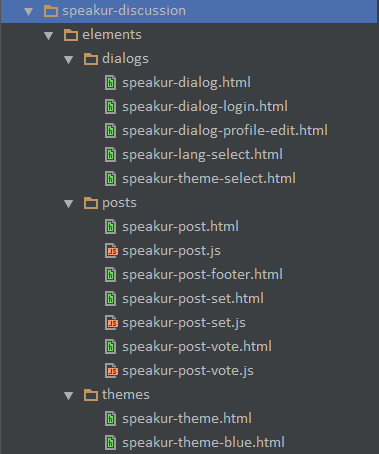
\includegraphics[width=\textwidth]{images/file_layout_a.png}
	\end{subfigure} %
	\begin{subfigure}[b]{0.48\textwidth}
		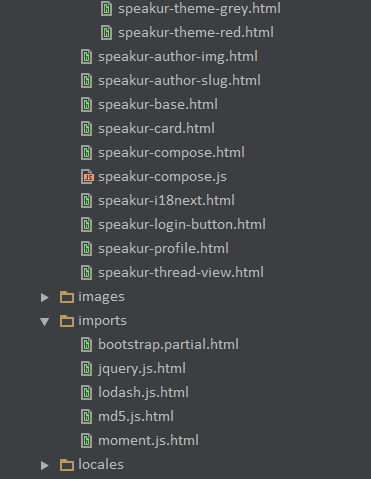
\includegraphics[width=\textwidth]{images/file_layout_b.png}
	\end{subfigure} %
	}
	\caption{Internal elements file layout (partial).}
	\label{f:file_layout}
\end{figure}

In addition to structural and logical elements, 
Speakur has a number of user interface (UI)\index{user interface (UI)} custom elements to do things like display an individual user post or show the post composition editor.
Elements are also reused extensively in different contexts; 
for example \tcode{<speakur-post>} is used for a `live editor preview' inside \tcode{<speakur-compose>} as well as for showing posts in the main \tcode{<speakur-thread-view>.}

Some of Speakur's internal components like \tcode{<speakur-theme>} are also base clas\-ses for other elements
in a way that is similar but not identical to classes in object oriented programming (OOP)\index{object oriented programming (OOP)}\footnote{Note that JavaScript\index{JavaScript} itself is \textit{prototype}-based\index{prototype (JavaScript)} and does not have traditional classes or inheritance. 
Similar behavior is obtained by using regular object instances (instead of classes) as the prototype for instantiating new objects.}. 
Although composition\index{composition} or \textit{has-a} relationships are generally preferred, inheritance\index{inheritance} or \textit{is-a} relationships can make sense when you truly want to be able to substitute one instance for another interchangeably.
JavaScript does not have the concept of a formal interface contract, which puts the burden of type checking on developers and unit tests,
but HTML elements (including custom elements\index{Custom Elements}) have formally specified interfaces\index{API} in the form of declared attributes.

\section{Database Design}
\label{sec:database}

Speakur uses Firebase for NoSQL\index{NoSQL}-style database storage.
Traditional relational databases\index{relational database} (SQL\index{SQL}) have emphasized data normalization\index{normalization (database)} -- the removal of informational redundancies from databases such that a given \textit{fact} is only recorded in a single place.
While this helps ensure data integrity, it can adversely affect query time and scalability as additional joins are required to bring in the necessary facts.
One of the defining characteristics of the NoSQL movement is denormalization\index{denormalization}---that is, the principle of eliminating redundancy is sacrificed in order to gain performance~\cite{sadalage2012}.
Facts can be defined in more than one place to speed up queries by reducing the number of read operations.

For example, some information about a post's author 
such as their public username, id, and photo url is saved inside each post they write 
so that it's not necessary to look up this information separately just to display the post.
One consequence of this is that changing your public name doesn't retroactively change the name on all of your previous posts, just new posts going forward.
Certainly, if that name updating was deemed necessary according to business requirements it could be accomplished.

% p{8cm}
\begin{table}\centering
\ra{1.3}
\begin{tabular}{@{}lll@{}}
\toprule
Table Name & Function & Key Structure \\
\midrule
\tcode{admins} & Administrator authorizations & \tcode{\$uid} \\
\tcode{posts} & User posts & \tcode{\$parent->\$child} \\
\tcode{postvotes} & Public vote counts for posts & \tcode{\$parent->\$child} \\
\tcode{profile} & User data and preferences & \tcode{\$uid} \\
\tcode{threads} & Discussion thread definitions & \tcode{\$threadId} \\
\tcode{uservotes} & User votes for posts & \tcode{\$uid->\$parent->\$child} \\
\bottomrule
\end{tabular}
\caption{Speakur's database tables.}
\label{table:speakurtables}
\end{table}

The logical interface presented by Firebase\index{Firebase} resembles a single JavaScript\index{JavaScript} object which can contain other objects and lists nested up to 32 levels deep~\cite{firebasecontributors2015}.
A JavaScript object is fundamentally a \tcode{key->value} mapping, also known as a hash map or (in Python\index{Python language}) as a dictionary.
Although this nested object structure doesn't correspond exactly to traditional relational database\index{relational database} (SQL\index{SQL}) tables, 
it is convenient to refer to the top (first) level of nested objects as ``tables''.
The leaf node objects are ``records'' with data fields, and the intermediate objects are keys within the table.
Like most NoSQL databases, Firebase is forgiving with regard to structure and fields; 
a given record is not guaranteed to follow any particular structure unless this is required by the security and validation rules.

\begin{figure}[htb]
\centering
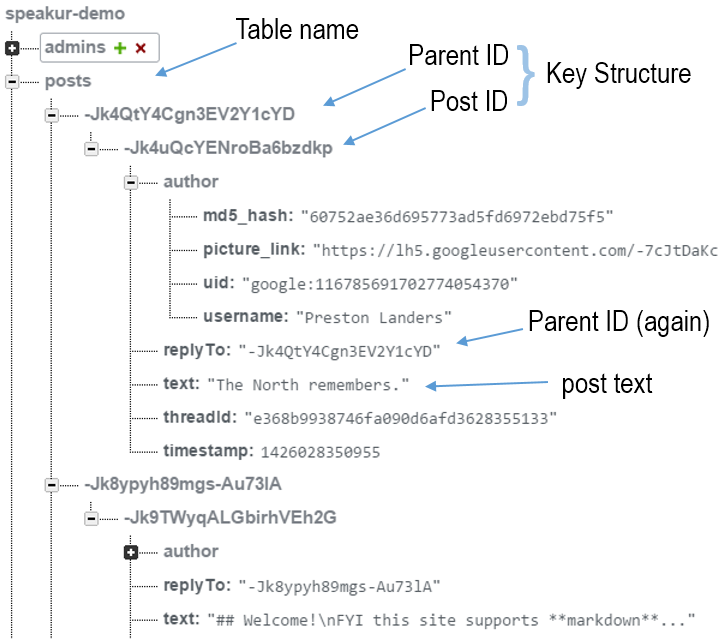
\includegraphics[width=0.93\textwidth]{images/firebase_admin_posts_b.png}
\caption{Structure of the \tcode{posts} table.}
\label{f:firebase_admin_posts}
\end{figure}

The key structure column in~\cref{table:speakurtables} signifies the meaning of the keys underneath a table. 
For example, the main \tcode{posts} table has a \tcode{\$parent->\$child} key structure.
The first layer of keys beneath \tcode{posts} are post \textit{parent} ids: 
the id of the post that this is a reply to,
or the thread id in the case of a `top-level' post.
The next object down the key hierarchy is the \textit{child} id, 
which is the id of the actual post itself.
The keys beneath that are the `fields' of the table, 
such as the \tcode{text} and \tcode{replyTo} values.
\Cref{f:firebase_admin_posts} shows Firebase's administrative view of the database.
The \tcode{posts} table is expanded, 
showing the parent and child id layers and the actual post object nested within.
Deeply nested data structures are not good for scalability; 
relatively flat tables are best~\cite{firebasecontributors2015,sadalage2012}.
The key structure will become important when we apply security rules in~\cref{sec:security}.


In addition to denormalizing\index{denormalization} the data as necessary, sometimes it is convenient for security reasons to 
keep related bits of data in separate tables in order to apply different security rules.
For instance, we want users to be able to modify a post's vote count without being able to modify the post itself.
The nested and denormalized\index{denormalization} structure of the tables helps ensure that we only fetch what we need, when we need it.
The flip side is that we need to be aware of these data duplications and update them as necessary, 
which can be difficult in a more sophisticated application.
But in the post vote count example, even if a malicious user sets a false count on the globally-visible value,
we can always recalculate the true count later using the individual user vote records.

\section{Component Synchronization}
\label{sec:sync}

Speakur\index{Speakur} consists of a number of Polymer\index{Polymer} components which break down the problem of presenting a discussion forum into smaller tasks.
Some of these components are listed in~\cref{table:speakurcomponents} on~\cpageref{table:speakurcomponents}.
They form a hierarchy with \tcode{<speakur-discussion>}\index{<speakur-discussion>} at the top (root). 
\Cref{f:component_layout} illustrates this, with many components omitted for brevity.

\begin{figure}[htb]
	\centerline{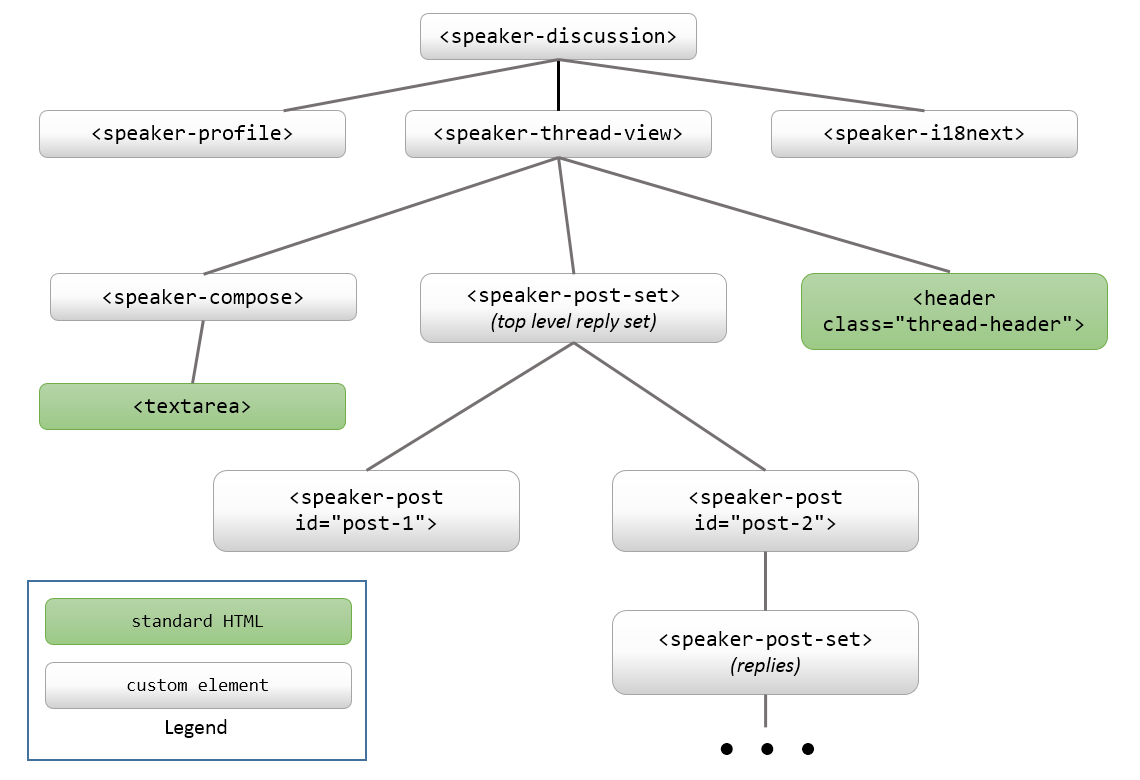
\includegraphics[width=6in]{images/components.png}}
	\caption{Speakur component hierarchy (partial).}
	\label{f:component_layout}
\end{figure}

The general data flow is that bindings carry information \textit{down} from parent to child, and changes flow \textit{up} in the form of events and observed mutations.
Two-way bindings are possible in that a child element can modify a bound variable and the value would be reflected in the parent and vice-versa, 
but in some scenarios this makes it difficult to determine an `authoritative' value 
or causes other circularity problems.
For this reason, bindings should be used one-way across component lines,
but two-way bindings are useful within a component to update its data model automatically from user input~\cite{polymercontributors2015-b}.

Each component keeps its own \tcode{<firebase-element>} to pull data from Firebase\index{Firebase} as needed,
or in some cases the relevant object is passed in as a binding from a parent element that has its own \tcode{<firebase-element>}.
This keeps database specific knowledge localized to each component, helping it ``be composable''.
Speakur\index{Speakur} as a whole doesn't know or care what storage solution its individual components use, whether Firebase\index{Firebase} or another API\index{API}.

\subsection{Data Bindings and Events}
\label{sec:databindings}
From an MVC\index{model-view-controller} viewpoint, a Polymer element with instance variables is the `model'.
The element's data-bound\index{data-bound template} \tcode{<template>}\index{<template>} is the `view', 
and the JavaScript\index{JavaScript} code is the `controller'.
Data bindings carry data information down from parent to child while DOM\index{DOM} events\index{event notification} propagate upwards.

Using \tcode{<firebase-element>} isolates each component from direct interaction with the general purpose Firebase\index{Firebase} JavaScript library
and ties the database directly into the Polymer\index{Polymer} data binding system.
Persisting a change is incredibly easy; 
writing a new value to a variable not only saves it to the database but pushes the change
to all other `subscribers'---whoever is viewing that post or other object at the time.
The \tcode{data=} attribute on 
\tcode{<firebase-element>}
allows binding a variable in a component to a remote database object:

\begin{lstlisting}[language=HTML5,caption={Binding the \tcode{post} variable to a database record.},label=l:fb_bind,captionpos=below]
<!-- from speakur-post.html -->
<firebase-element
   data="{{ post }}"
   location="{{ fbLocation(firebaseLocation, 'posts', parentId, postId) }}">
</firebase-element>
\end{lstlisting}

In the example above, 
the data retrieved by the \tcode{<firebase-element>}
is bound by the \tcode{\{\{ \}\}} operators to the component's \tcode{post} variable. 
Any changes to this database object, 
whether locally or remotely initiated,
will be reflected in the \tcode{post} variable
and any associated data-bound\index{data-bound template} \tcode{<template>}\index{<template>}s, 
and vice-versa.
The \tcode{location=} attribute (the database source URL) for this \tcode{<firebase-element>}\index{<firebase-element>|)}
is bound to an expression which finds the location with the \tcode{fbLocation} method.
Any changes in the variables \tcode{firebase\-Location}, \tcode{parentId} or \tcode{postId} will cause \tcode{fbLocation} to be recomputed,
which could in turn cause \tcode{post} to pull from a different location.
Notice that \tcode{location=} has the same structure as the resource path in the \tcode{DELETE} example from~\cref{l:rest_delete}.

DOM events carry state changes up from children to elements above it.
Polymer provides the \tcode{fire()} method to trigger a named event with extra data attached.
This is a convenience wrapper since it can be done with pure JavaScript\index{JavaScript}.
An example of using \tcode{fire()} can be found in the language selection dialog from~\cref{f:lang}.
The language selection UI is handled in the \tcode{<speakur-lang-select>} component,
which is only concerned with presenting the language chooser and not with handling the actual localization,
reinforcing separation of concerns.
When the user selects a new language it fires an event that bubbles up to the top level \tcode{<speakur-discussion>} element:

\begin{lstlisting}[language=JavaScript,caption={Firing a language change event.},label=l:fire_event,captionpos=below]
// from speakur-lang-select.js
domReady: function () {
    // listen for core-select event fired by the dropdown menu
    this.$.menu.addEventListener('core-select', function (e) {
        if (e.detail.isSelected) {
            var oldLocale = this.locale;
            var newLocale = e.detail.item.id;
            
            // Tell container(s) the language selection changed
            this.fire('speakur-locale-change', 
               {oldLocale: oldLocale, newLocale: newLocale});
        }
    });
}
\end{lstlisting}

A handler in the top level container (\tcode{<speakur-discussion>}\index{<speakur-discussion>}) responds to this named event (\tcode{speakur-locale-change}) and tells the
internationalization\index{internationalization} component to update the language.
This in turn sets the \tcode{\textbf{lc}} (locale) property in the base element.
This property is then used in translation expressions as discussed in~\cref{sec:i18n}.

\subsection{Data-Bound Templates}
\label{sec:dbtemplates}
Speakur translates internal variables (the model) into visible output with the use of data-bound templates\index{data-bound template}.
This is similar in effect to the model-view-controller\index{model-view-controller} design pattern.
As mentioned above, the custom element itself is the `model' and its \tcode{<template>}\index{<template>} is the view.
This allows embedding variables directly in the HTML\index{HTML} representation of a component as shown in~\cref{l:dbtemplate} on~\cpageref{l:dbtemplate} and here:

\begin{lstlisting}[language=HTML5,caption={User interface control with data bindings (edit post link).},label=l:bind_ui,captionpos=below]
<!-- from speakur-post-footer.html -->
<div on-click="{{editPost}}" hidden?=
    "{{!canEditPost(post, globals.profile, globals.isAdmin)}}">
  {{ "Edit" | $$(lc) }}
</div>
\end{lstlisting}

There are three data bindings with \tcode{\{\{ \}\}} in~\cref{l:bind_ui}:
\begin{enumerate}
\item The \tcode{hidden?=} attribute (provided by Polymer\index{Polymer}) binds to \tcode{canEditPost} to determine if the Edit link should be shown under a post. 
In other words, is this user allowed to edit this post? If not, hide this Edit \tcode{<div>}.
\item The \tcode{<div>} binds its click event to \tcode{editPost} so it functions as a link. The \tcode{editPost} method of this component will be called when the Edit link is clicked.
\item The inner content of the \tcode{<div>} (its light DOM) is bound to a Polymer filter expression that translates the word ``Edit'' to the current language. 
\end{enumerate}

The \tcode{\{\{ \}\}} operators are not limited to binding to simple variables.
Polymer supports a rich expression language within binding operators. 
That said, keeping \tcode{<template>}\index{<template>} expressions simple and moving more complex logic to methods in the JavaScript\index{JavaScript} controller helps uphold separation of concerns between controller and view.

\section{Data Security}
\label{sec:security}
Because Firebase\index{Firebase} is Speakur's only `server', 
most of its security\index{security} rests in Firebase's authentication\index{authentication} and authorization\index{authorization} rules.
Obviously the user interface should be crafted such that undesirable actions are not presented as options for the user,
but one also has to consider malicious users stepping outside of the allowed interface
and/or directly accessing the REST\index{REST} API\index{API}.
Authentication\index{authentication} ensures that we know the identity of anyone making database changes,
and the Firebase\index{Firebase} security rules enforce authorization\index{authorization} requirements.

\subsection{OAuth Authentication}
Speakur\index{Speakur} supports signing in (authenticating\index{authentication}) users with two popular single sign-on services: Google\index{Google} and Facebook\index{Facebook}.
This avoids the need to create a dedicated user registration and password system.
In this scenario, Google or Facebook is an OAuth\index{OAuth} identity provider (IdP),
and Firebase\index{Firebase} (standing in for Speakur) is a service provider (SP).
The identity provider gives the service provider a limited selection of personal information, generally their name, profile picture, and email address.
The user authenticates directly to the chosen IdP (e.g. Facebook\index{Facebook}) and their password is never sent to Firebase or Speakur\index{Speakur}.
Future versions may support additional identity providers like GitHub\index{GitHub} and Twitter\index{Twitter} as well as Firebase's\index{Firebase} own simple user registration system.

Inside Speakur, authentication is handled by the \tcode{<firebase-login>} element, provided by \tcode{<firebase-element>}~\cite{polymercontributors2015-c}.
A binding is set up between that and the \tcode{user} variable in \tcode{<speakur-discussion>}\index{<speakur-discussion>} so that when user authentication is completed, the \tcode{user} variable contains an object with user properties like their full name and authentication ID.
The authentication\index{authentication} session is automatically used by any \tcode{<firebase-element>} anywhere on the page provided that their \tcode{location=} points to the same database base URL.

\subsection{Firebase Security Rules}
\label{sec:fbsecurity}

Authorization to perform any given action in the Speakur\index{Speakur} database is determined by consulting the nested rules in the 
JSON-formatted\index{JSON} security\index{security} object, 
whose documentation can be found at~\cite{firebasecontributors2015-a}.
These rules can be entered directly into the Firebase\index{Firebase} administrative console
and a reference copy can be found in the Speakur\index{Speakur} source code repository under the file \tcode{security-rules.json}~\cite{landers2015-c}.
These rules are enforced by the Firebase service itself, not my application code.

The structure of the security rule object mirrors the nested hierarchy of the Firebase database itself.
Each top level key maps to rules for a particular database ``table'' like \tcode{posts}.
These fall into three categories: read, write, and validation rules.
These are each structured as boolean expressions (predicates) that determine whether the given action is allowed.
Example rules are given in~\cref{l:sec_rule1} on~\cpageref{l:sec_rule1}.

\begin{enumerate}
\item \tcode{.read} rules determine whether a given record can be retrieved by the current user.
\item \tcode{.write} rules authorize the creation, modification and deletion of a record.
\item \tcode{.validate} rules check whether a record is correctly \textit{structured}.
\end{enumerate}

Write rules determine whether a given create, modify or delete is allowed. 
Validate rules are run after a write rule has passed in order to check whether the new version is correctly structured per business rules or requirements.
Each expression has access to several pre-defined variables including snapshots of the database as it exists both before and after the change would be applied.
For example,~\cref{l:sec_rule1} (\cpageref{l:sec_rule1}) shows rules for the \tcode{posts} table.
The \tcode{.write} rule asserts that anyone can create a new post, 
but modifying an existing post requires that you (\tcode{auth.uid}) are either the post owner or an administrator.
The \tcode{.validate} rule ensures that all posts contain at least 4 keys: \tcode{threadId}, \tcode{text}, \tcode{author}, and \tcode{timestamp}.
More sophisticated rules and validations are possible, and rules can be nested, 
but it can be unwieldy to fit a large set of rules into a single predicate expression, 
making them more difficult to understand and maintain.

\section{Internationalization and Localization}
\label{sec:i18n}
Adapting an application for different languages and customs is called internationalization\index{internationalization|textbf} (i18n) and localization\index{localization|textbf} (l10n)\footnote{\textit{Internationalization} refers to the process of \textbf{enabling} an app to be localized, and \textit{localization} refers to adapting it to a \textbf{specific} locale.
}. 
Speakur\index{Speakur} offers UI translations for 15 languages.
The user can select a new language from the Profile dialog and the interface updates immediately.
String substitution with the currently selected language is handled by the i18next\index{i18next library} JavaScript library, 
which is abstracted\index{abstraction} with a custom element wrapper \tcode{<spe\-akur-i18\-next>}~\cite{i18nextcontributors2015}.
This wrapper provides a Polymer filter named \tcode{\$\$} which is used in \tcode{\{\{ \}\}} expressions in data-bound templates\index{data-bound template} to translate user-visible UI strings.
Of course, the users' posts themselves are not translated; just the application's interface strings.

The i18next library loads strings out of JSON\index{JSON} files, one for each supported language.
I obtained translations by creating an English language file and then passing it through the Microsoft\index{Microsoft} Translation API\index{API} using `Eurgh!'\index{Eurgh (translation library)},
a Python\index{Python language} program that I wrote for another project~\cite{landers2015-a}.
The i18next library includes variable interpolation (insertion points for data) and pluralization rules that are important for grammatically correct text.
Here is a short excerpt from the English file followed by the Russian version:

\begin{lstlisting}[language=JavaScript,caption=
{String resources for internationalization\index{internationalization|textbf}.},label=l:i18n,captionpos=below]
// from speakur-en.json
{
  "View Comments": null,
  "replies_count": "__count__ reply",
  "replies_count_plural": "__count__ replies"
}
// from speakur-ru.json
{
  "View Comments": "Посмотреть комментарии",
  "replies_count": "ответ __count__",
  "replies_count_plural": "__count__ ответы"
}
\end{lstlisting}

%   "apples_oranges": "Mary has __apples__ apples and __oranges__ oranges.",
%    "apples_oranges": "Мэри имеет __apples__ яблоки и апельсины __oranges__.",

This example shows that with the \tcode{'View Comments'} key, the corresponding value can be null if the key itself can serve as the text. 
The other two keys illustrate variable interpolation and pluralization logic where different grammatical forms can be selected based on a numeric variable, 
in this case, the number of replies that a post has.
These translation strings would be used in a template like:
%\pagebreak
\begin{lstlisting}[language=HTML5,caption={Internationalizing\index{internationalization|textbf} a data-bound template.},label=l:i18n_template,captionpos=below]
<!-- from speakur-post.html -->
<div class='post-replies-count'>
  {{ 'replies' | $$({count: replyCount}, lc) }}
</div>
\end{lstlisting}

The \tcode{i18next}\index{i18next library} library sees that a \tcode{count} variable is provided to \tcode{\$\$} and looks for that key (\tcode{rep\-lies}) with either a \tcode{\_count} or a \tcode{\_count\_plural} suffix depending on the cardinality of \tcode{count}.
In this expression the \tcode{lc} variable (the second parameter to the \tcode{\$\$} call) reflects the user's current language setting, such as \tcode{lc=en} for English or \tcode{lc=ru} for Russian.
Interestingly, the \tcode{lc} variable is \textit{not} required by the \tcode{\$\$} filter because it already knows the current locale.
Instead, \tcode{lc} is included in the expression merely to register a value dependency with Polymer\index{Polymer}
such that when the locale is changed elsewhere, all dependent expressions are recalculated, or in this example, the strings are re-translated to the current 
locale\footnote{Polymer expression dependencies are implemented internally with DOM mutation observers\index{mutation observers}~\cite{polymercontributors2015-b}.}.
In this case it would output something like ``1 reply'' or ``2 replies'' as needed.
Otherwise Polymer\index{Polymer} wouldn't bother to recalculate this expression when the locale (\tcode{lc}) changed because none of its direct clauses had acquired different values.
Adding \tcode{lc} to this expression ensures that the text is updated when the language changes.

%\subsection{Architecture}
%\subsection{Libraries}

Another powerful internationalization\index{internationalization|textbf} feature is provided by the moment.js library\index{moment.js library}, 
a general purpose date/time library that also provides date-related localization\index{localization} services.
Unlike the general UI strings, the date translations are not provided by Speakur\index{Speakur}, but are included in moment.js itself.
In addition to formatting dates and times (like the time of a post) according to local conventions, 
it also provides a \tcode{fromNow} function that outputs a localized ``ago'' string---the amount of time elapsed since a certain point such as ``10 seconds ago'' or ``3 weeks ago''.
Speakur\index{Speakur} uses this in post headers to show how long ago they were posted,
and ties them to a timer-based value dependency such that the ``ago time'' updates automatically on the page as time passes. 
For example, immediately after posting a new reply, its header will say ``posted a few moments ago.'' 
After a minute it will say ``posted a minute ago'', and so on in idiomatic fashion appropriate to the current language.
This text has a tooltip which gives the full localized date such as ``Wednesday, March 11th 2015 7:53 pm''.

\section{Device-Responsive Design}
\label{sec:responsive}
As mentioned in~\cref{bg:mobile}, Speakur\index{Speakur} uses several techniques to achieve a design that automatically responds\index{responsive design} to different devices and screen sizes, 
including mobile phones.
The three main responsive design techniques used in Speakur are:
\begin{enumerate}
\item Using CSS\index{CSS} \tcode{@media}\index{@media} rules to apply different styles such as sizes and margins to different screen sizes.
\item Using CSS Flexible boxes (a.k.a. `flex') layout with \tcode{wrap} options to create structures like toolbars while allowing them to gracefully rearrange on smaller screens.
\item Using a JavaScript variable (\tcode{smallScreen}) to control the behavior of data-bound templates\index{data-bound template} and provide a different experience on smaller devices.
\end{enumerate}

In Speakur's style sheets, a small screen is treated as the base case and 
larger tablet or desktop-style devices are given extra rules with \tcode{@media}.
For example, the following rule gives the main Speakur container more padding on large screen devices:
%\pagebreak
\begin{lstlisting}[language=HTML5,caption={CSS @media rule for large screen devices.},label=l:responsive_media,captionpos=below]
<!-- from speakur-discussion.css -->
@media only screen and (min-device-width : 800px) {
  :host .speakur-body-container {
    margin: 4px;
    padding: 8px;
  }
}
\end{lstlisting}

In summary, CSS Flexible boxes\index{Flex} let you give \tcode{<div>} and other elements `flex layout' attributes that provide guidance to browsers about how to align the contents inside and adjust for available space.
Polymer\index{Polymer} provides convenient layout shortcuts for the standard CSS attributes~\cite{polymercontributors2015-d}.
%For example, the following sets up a `header' with the equally 

%\begin{lstlisting}[language=HTML5,caption={CSS\index{CSS} Flexible boxes\index{Flex} for device-responsive\index{responsive} layout.},label=l:responsive_flex,captionpos=below]
%<!-- from speakur-thread-view.html -->
%\end{lstlisting}

\section{Publishing and Deployment}
\label{publishing}

Speakur\index{Speakur} is published to \tcode{github.io}, 
a static web host and content delivery network for GitHub\index{GitHub} projects.
This allows users to import the component without hosting it themselves.
Web authors can also host Speakur's files on their own server if desired.
This makes it very easy to deploy\index{deployment} Speakur in a wide variety of system architectures.
Speakur\index{Speakur} is provided in two versions; 
the `development' version where each resource is provided as a separate, raw, non-minified\index{minify} file,
and a `production' or Vulcanized\index{Vulcanize} version where all necessary resources are combined into a single file for faster loading speeds~\cite{polymercontributors2015-a}. 

In a relatively small application like Speakur the difference is not huge, especially on Google Chrome\index{Google!Google Chrome} which already supports Web Components natively,
because the HTML component transfer times are largely dwarfed by the cost of loading the actual discussion from the database.
Future protocol enhancements like HTTP 2\index{HTTP!HTTP 2.0} may eliminate this discrepancy.
That said, using Vulcanize does offer current benefits,
as shown in~\cref{table:speakurloading} which compares the time (in milliseconds) to initially display the Speakur component and then fully load a thread with 25 comments in three popular desktop browsers.
These figures partly reflect the degree to which each of these browsers natively supports Web Components\index{Web Components} at this time.
At the moment Firefox\index{Mozilla!Mozilla Firefox} does not natively support as many Web Component features as Google Chrome\index{Google!Google Chrome} or Opera\index{Opera}, 
so the polyfill\index{polyfill} must do more work, negatively impacting load times on that browser.
I expect that browser support will improve greatly over the next few years after the Web Components standard is finalized.

% p{8cm}
\begin{table}\centering
\ra{1.3}
\begin{tabular}{@{}lrrr@{}}
\toprule
State & Raw & Vulcanized & Reduction \\
\midrule
\textbf{Google Chrome}\index{Google!Google Chrome} \\ 
visible & 2200 & 1150 & 47.7\% \\
complete & 4200 & 2900 & 31.0\% \\
\\
\textbf{Mozilla Firefox}\index{Mozilla!Mozilla Firefox} \\ 
visible & 7400 & 6050 & 18.2\% \\
complete & 12000 & 10500 & 12.5\% \\
\\
\textbf{Opera}\index{Opera} \\ 
visible & 2800 & 1100 & 60.7\% \\
complete & 7000 & 2800 & 60.0\% \\
\bottomrule
\end{tabular}
\caption{Loading time (in milliseconds) in three desktop browsers.}
\label{table:speakurloading}
\end{table}


\chapter{Analysis and Lessons Learned}
\index{Analysis and Lessons Learned%
@\emph{Analysis and Lessons Learned}}%
\label{ch:analysis}

This report aims to demonstrate how certain traditionally difficult problems in web development have been addressed by Web Components\index{Web Components}.
The principles underlying Web Components and Polymer\index{Polymer} are summarized by the list in~\cref{sec:wcprinciples} taken from ~\cite{webcomponentscontributors2014}.
I have tried to make Speakur\index{Speakur} adhere to these principles both internally and externally,
and to demonstrate the application of abstraction\index{abstraction} and encapsulation\index{encapsulation} patterns to creating flexible, composable, reusable, sharable components.
My goal is to understand how the W3C Web Component\index{Web Components} initiative will impact web application engineering\index{software engineering} in the future.
By all appearances, the long term impact will be substantial.

\section{Web Components Architecture Analysis}
Web Component's\index{Web Components} essential benefit is that it allows decoupling of components, 
separation of concerns, 
and the encapsulation of internal structure.
This raises bundles of discrete functionality or `components' to a higher level of abstraction and 
will help open up a new ecosystem of reusable, extendable, sharable modules.
The Web Component principles from~\cref{sec:wcprinciples} emphasize thinking small, 
breaking the problem down into manageable chunks and being adaptable, extendable and composable.
Web developers were already doing this in many cases, but without formal support from the browser.

Perhaps the most interesting piece of advice is to ``deliver the key benefit to HTML authors, not just coders''~\cite{webcomponentscontributors2014}.
It underscores that, fundamentally, 
the web consists of \textit{documents} with \textit{authors}, 
a fact that is sometimes forgotten by the myriad of JavaScript\index{JavaScript} libraries and frameworks\index{framework}.
The components that will find the most success will be those which focus first and foremost on providing convenience and benefit to HTML\index{HTML} authors and content developers, 
not just the software engineers\index{software engineering} who maintain the libraries and frameworks behind the scenes.
Speakur\index{Speakur} aims to provide as small a deployment surface as possible to web authors so they can easily add a discussion forum to their site without embedding a big blob of HTML.
The growth of social coding sites like GitHub\index{GitHub} will further encourage the sharing and reuse of Web Components designed along these principles.

\section{Writing Web Components with Polymer}
This section details some of the lessons learned developing Speakur\index{Speakur} on top of Google's\index{Google} Polymer\index{Polymer} framework.

\subsection{Using Data-Bound Templates}
Polymer's data bindings\index{data-bound template} are a powerful feature for driving `live' web applications.
Their utility extends well beyond user interface\index{user interface (UI)} views.
A 3-way automatic binding between the local model, the UI view, and the remote database is an extremely powerful abstraction,
even more so when combined with Firebase's\index{Firebase} 
Web\-Socket-based\index{WebSockets} event notification\index{event notification} system.
JavaScript variables can automatically update to reflect changes made by users on the other side of the world.
Of course, care must be taken to design the interface so the user doesn't accidentally make changes that are immediate and can't be undone. 
For example, Speakur's user preferences screen doesn't commit changes to the database until the user clicks the Save button.
Editing the text of an existing post also saves a copy of the previous version.

\subsection{Decoupling Components}
Data bindings and synchronization are discussed in~\cref{sec:sync}.
In general, two-way data bindings should only be used \textit{within} a component.
Across component boundaries, use a one-way binding to send data down to a child,
and fire events to notify containers of state changes.
DOM Mutation Observers\index{mutation observers} can be useful for making one component react to a change in another without directly tying their code together.
As the example with \tcode{lc} (locale) in~\cref{sec:i18n} showed, 
sometimes it is necessary to `shoehorn' certain variables into a Polymer binding expression 
to ensure that the expression is recalculated when that variable changes.

\subsection{Optimizing Polymer Performance}
Component load times are currently one problem area for Web Components.
The Vulcanize\index{Vulcanize} tool offers definite benefits for load times as seen in~\cref{table:speakurloading},
but Speakur is a relatively simple application where all 20 or so components are used more or less immediately.
The Vulcanize tool must be applied at the level of the site or app, not by the individual component authors.
Larger single page applications (SPAs) will face more complex challenges when trying to optimize load times, and performance in general,
before Web Components\index{Web Components} are fully native in browsers, especially when combining frameworks.

The \tcode{<template>}\index{<template>} element is a powerful new tool for web authors, 
but current implementations can have performance issues when rendering large lists of items, such as with a long list of comments. 
Polymer's\index{Polymer} \tcode{<core-list>} is more optimized for this use case.
Also, the \tcode{if=} attribute on nested \tcode{<template>}\index{<template>} elements should not be used in those cases where you could use the \tcode{hidden?=} attribute on the inner content instead.
There are several reasons for this, including performance and 
the fact that Polymer's handy \tcode{this.\$} \tcode{id}-to-object map is not dynamic; 
that is, element objects created conditionally in inner templates are not automatically added to \tcode{this.\$}.

\subsection{Inheritance in Polymer}
I recommend avoiding the use of Polymer's\index{Polymer} inheritance unless there is a clear case for providing polymorphism-like\index{polymorphism} behavior.
One reason for that is that (as of this writing) when a base class provides computed properties, 
these property definitions have to be repeated in any subclasses if any new ones are required,
which violates the ``don't repeat yourself'' (DRY)\index{don't repeat yourself (DRY)} principle.
Speakur uses Polymer inheritance\index{inheritance} in its CSS\index{CSS} theme components; 
most of the functionality is defined in the base class and the subclasses mainly provide numeric parameters for things like colors and margins.
Composition\index{composition} could achieve these behaviors almost as easily.

%Having multiple <core-overlay> active at the same time can cause problems. 
% I created a simple fix that adjusts the CSS \tcode{z-index} property. 
%You can find the fix here:~\cite{landers2015-d}.

\section{The Future of Web Components}

Polymer\index{Polymer} and Web Components\index{Web Components} are extremely powerful tools.
They are relatively immature as a technology but quickly improving.
Those who wish to deploy a large, full-featured ``prod\-uction-quality'' web application based on these technologies may face some bumps in the road, 
at least until the standard is finalized and browser support is improved.
A project version below 1.0 is a general indicator of how ready its authors feel it is for production deployment, and Polymer's\index{Polymer} current version is at 0.5, soon to be 0.8, 
which suggests that 1.0 is not that far off.
Even the massively popular Angular\index{Angular} framework has announced that the controversial 2.0 re-write will be based on the Web Components standard,
so it appears that Web Components are here to stay~\cite{santiagoesteva2015}.

The Web Components\index{Web Components} initiative is much bigger than just the Polymer project.
The draft is due to be formally adopted as an official HTML5\index{HTML!HTML5} standard by the World Wide Web Consortium\index{W3C}.
Although it will still be a long time before full-speed native Web Component support is found in a majority of browsers worldwide, 
polyfill\index{polyfill} libraries can help bring these capabilities to current browsers.
However the prospect of forcing visitors to download a several hundred KB library just to use basic DOM functionality is not very appealing to most web engineers from a performance and user experience\index{user experience (UX)} perspective, 
so the lack of native browser support may be a limiting factor in Web Component adoption in the near term.

In essence, Web Component's\index{Web Components} key problem at the moment is that one has to download a large JavaScript\index{JavaScript} framework\index{framework} in order to use it, 
yet one of its main premises is that it frees you from needing a JavaScript framework.
Of course, the path out of this chicken-and-egg problem is for browser vendors to fully implement native Web Components in their products,
a process which won't be complete until well after the standard is finalized by the W3C.
Given the enormous size of the job that the polyfill library must accomplish, the results obtained so far are impressive. 
Speakur\index{Speakur} has demonstrated that it's possible to create focused, extensible, yet full-featured Web Components right now with the help of tools like Polymer\index{Polymer} and Firebase\index{Firebase}.


\chapter{Conclusion}
\index{Conclusions%
@\emph{Conclusions}}%

Web Components\index{Web Components} are a powerful addition to the web developer's arsenal. 
Their fundamental premise is that web content can be componentized, encapsulted\index{encapsulation}, and abstracted\index{abstraction} behind well-defined APIs\index{API}.
Eventually this functionality will be delivered directly by the browser without needing a dedicated JavaScript\index{JavaScript} framework.
%But for the immediate future, using Web Components in your application means that your clients must download a large blob of JavaScript library code -- the polyfill\index{polyfill} --- 
%that enables Custom Elements\index{Custom Elements}, 
%shadow DOM\index{Shadow DOM}, 
%templates\index{HTML!Templates}, and 
%the component import system\index{HTML!Imports}.
But for the immediate future, using Web Components in your application means that your clients must download a large blob of JavaScript library code---the polyfill\index{polyfill}---to enable its features: 
Custom Elements\index{Custom Elements}, 
shadow DOM\index{Shadow DOM}, 
templates\index{HTML!Templates}, and 
the component import system\index{HTML!Imports}.

Web Components have set out on the right path to becoming a mature, widely deployed technology. 
Newer frameworks like Polymer\index{Polymer} provide powerful abstractions but are still undergoing rapid evolution.
Older, more established frameworks like Angular\index{Angular} have already begun the process of adapting to the new Web Component world. 
Success will be found at the end of this road as long as framework and component authors remain mindful of the guiding principles of Web Components: 
to be small, focused, extensible, adaptive, 
and most of all, 
to deliver the key benefits 
not only to the software engineers\index{software engineering} who make the web run,
but to the content \textit{authors} that have made it the indispensable communications medium of the modern age.



%%%%%%%%%%%%%%%%%%%%%%%%%%%%%%%%%%%%%%%%%%%%%%%%%%%%%%%%%%%%%%%%%%%%%%
% Appendix/Appendices                                                %
%%%%%%%%%%%%%%%%%%%%%%%%%%%%%%%%%%%%%%%%%%%%%%%%%%%%%%%%%%%%%%%%%%%%%%
%
% If you have only one appendix, use the command \appendix instead
% of \appendices.
%
%\appendices


% http://tex.stackexchange.com/a/103173/75161
%\setcounter{table}{0}
%\setcounter{page}{1}
%\newcommand{\initAnhang}{
%    \renewcommand{\thepage}{A\arabic{page}}
%    \newpage
%}
%\renewcommand\appendix{\par
%        \renewcommand\thesection{A}
%        \renewcommand\thesubsection{A\arabic{subsection}}
%        \renewcommand\thetable{A\arabic{table}}}        
%\appendix\initAnhang


\appendix
\index{Appendices@\emph{Appendices}}%

%\chapter{Lerma's Appendix}
\index{Appendix!Lerma's Appendix@\emph{Lerma's Appendix}}%
The source \LaTeX{} file for this document is no longer quoted in
its entirety in the output document. A \LaTeX{} file can 
include its own source by using the command
\cn{verbatiminput\{\cn{jobname}\}}.



%%%%%%%%%%%%%%%%%%%%%%%%%%%%%%%%%%%%%%%%%%
\chapter{My Appendix \#2}
\index{Appendix!My Appendix \#2@\emph{My Appendix \#2}}%
\section{The First Section}
This is the first section.
This is the second appendix.

\section{The Second Section}
This is the second section of the second appendix.

\subsection{The First Subsection of the Second Section}
This is the first subsection of the second section of the second appendix.

\subsection{The Second Subsection of the Second Section}
This is the second subsection of the second section of the second appendix.

\subsubsection{The First Subsubsection of the Second Subsection of
		the Second Section}
This is the first subsubsection of the second subsection of the
second section of the second appendix.

\subsubsection{The Second Subsubsection of the Second Subsection
		of the Second Section}
This is the second subsubsection of the second subsection of the
second section of the second appendix.


% %%%%%%%%%%%%%%%%%%%%%%%%%%%%%%%%%%%%%%%%%%
\chapter{My Appendix \#3}
\index{Appendix!My Appendix \#3@\emph{My Appendix \#3}}%

\section{The First Section}
This is the first section.
This is the third appendix.

\section{The Second Section}
This is the second section of the third appendix.




\printindex{}

%%%%%%%%%%%%%%%%%%%%%%%%%%%%%%%%%%%%%%%%%%%%%%%%%%%%%%%%%%%%%%%%%%%%%%
% Generate the bibliography.					     %
%%%%%%%%%%%%%%%%%%%%%%%%%%%%%%%%%%%%%%%%%%%%%%%%%%%%%%%%%%%%%%%%%%%%%%
%								     %
% NOTE: For master's theses and reports, NOTHING is permitted to     %
%	come between the bibliography and the vita. The command      %
%	to generate the index (if used) MUST be moved to before      %
%	this section.						     %
%								     %
\nocite{*}      % This command causes all items in the 		     %
                % bibliographic database to be added to 	     %
                % the bibliography, even if they are not 	     %
                % explicitly cited in the text. 		     %
		%						     %

\begingroup
%\raggedright
%\sloppy
%\renewcommand*{\bibfont}{\raggedright}
\setlength{\bibitemsep}{6pt}
\printbibliography[heading=bibintoc]
\endgroup

%\bibliographystyle{plain}  % Here the bibliography 		     %
%\bibliography{diss}        % is inserted.			     %
\index{Bibliography@\emph{Bibliography}}%			     %
%%%%%%%%%%%%%%%%%%%%%%%%%%%%%%%%%%%%%%%%%%%%%%%%%%%%%%%%%%%%%%%%%%%%%%


%%%%%%%%%%%%%%%%%%%%%%%%%%%%%%%%%%%%%%%%%%%%%%%%%%%%%%%%%%%%%%%%%%%%%%
% Generate the index.						     %
%%%%%%%%%%%%%%%%%%%%%%%%%%%%%%%%%%%%%%%%%%%%%%%%%%%%%%%%%%%%%%%%%%%%%%
%								     %
% NOTE: For master's theses and reports, NOTHING is permitted to     %
%	come between the bibliography and the vita. This section     %
%	to generate the index (if used) MUST be moved to before      %
%	the bibliography section.				     %
%								     %
% \printindex%    % Include the index here. Comment out this line      %
%		% with a percent sign if you do not want an index.   %
%%%%%%%%%%%%%%%%%%%%%%%%%%%%%%%%%%%%%%%%%%%%%%%%%%%%%%%%%%%%%%%%%%%%%%


%%%%%%%%%%%%%%%%%%%%%%%%%%%%%%%%%%%%%%%%%%%%%%%%%%%%%%%%%%%%%%%%%%%%%%
% Vita page.							     %
%%%%%%%%%%%%%%%%%%%%%%%%%%%%%%%%%%%%%%%%%%%%%%%%%%%%%%%%%%%%%%%%%%%%%%

\begin{vita}
\renewcommand{\thefootnote}{\fnsymbol{footnote}}
Preston Brent Landers
was born in north Texas and attended high school on the Nevada side of Lake Tahoe. 
He received his Bachelor of Arts in English from the University of Texas at Austin with a minor in Government.
He works as a web and mobile software engineer for Journyx, Inc.\footnote[1]{\url{http://www.journyx.com}}
in Austin, Texas and began graduate studies in Software Engineering at 
the University of Texas at Austin in August 2012.

\end{vita}

\end{document}
